\documentclass[11pt]{article}
% =====================================================================
% [†ONT-BDRY] THE MATTER BOUNDARY — this paper is the HOME (ONTOLOGY_FOUNDATION_INDEX.md §1p).
%   THE REGISTER, FIXED AT THE OUTSET: "a negative result is as easy to overstate as a positive one."
%   WHAT IS ESTABLISHED IS BOUNDED: colour does not arise as a continuous internal gauge symmetry through
%   ANY EXAMINED GEOMETRIC-ISOMETRY ROUTE. THE UNIVERSAL CLAIM IS NOT MADE. Colour by the ordinary route —
%   an SU(3) matter bundle placed by hand — IS IN NO JEOPARDY AND IS NOT THE SUBJECT.
%   THE HARD CONSTRAINTS: (C2) su(3) is NOT in so(5,1), STRUCTURALLY — its smallest faithful real rep is
%   SIX-dimensional, so su(3) is in so(6) but not so(5), and so(5) is the maximal compact subalgebra of
%   so(5,1). "Colour needs a six-dimensional real carrier; the Lorentzian substrate's compact sector
%   supplies only five." (C3) WHERE su(3) CAN ACT GEOMETRICALLY, IT ACTS *SPATIALLY*, NOT INTERNALLY — it
%   acts transitively on S^5 = SU(3)/SU(2) and ADMITS NO EQUIVARIANT MAP TO THE COSMOLOGICAL S^3, so the
%   cut breaks it: "a symmetry of SPACE, which the physical cut destroys." (C7) su(3) lives ONLY on the
%   compact (Wick) face, reached OFF the real Lorentzian substrate by a change of signature.
%   *** THREE OPERATIONS ARE CO-LOCALISED AT THE SEAM r = sqrt(3/Lambda) — NEVER FUSE THEM:
%     (1) the REAL Weyl reflection sigma — fixes x_0, fixes BOTH signatures, FIXES THE GEOMETRY;
%     (2) the SEAM CONTINUATION theta -> pi/2 + i.psi — flips the signature of a SINGLE slicing curve,
%         reaching the equatorial S^4 with isometry SO(5);
%     (3) the GLOBAL WICK ROTATION x_0 -> i.x_0 — reaching S^5 with isometry SO(6) ⊃ su(3).
%   "ONLY THE LAST LANDS ON THE FACE WHERE su(3) LIVES." Reading sigma as the bridge conflates (1) with (3);
%   reading the seam continuation as the bridge conflates AN SO(5) OPERATION WITH AN SO(6) ONE. The
%   so(6)\so(5) generators su(3) needs are supplied by the global Wick and by NEITHER of the others. ***
%   THE CASCADE: colour is DROPPED the instant one descends to the real substrate ("'the gauge structure is
%   which isometry survives the real-substrate cut' returns GRAVITY, NOT GAUGE"). THE RANK COUNT: the SM
%   gauge group has RANK 4; SO(6) has RANK 3; a subgroup's rank cannot exceed the group's, SO THE WEAK SU(2)
%   DOES NOT FIT, and the raise to dS_6 buys AT MOST SU(3) x U(1) — "colour-plus-a-U(1), and the rest is a
%   TOWER OF POSITS." The A_2/S_3 skeleton is GENUINE and GEOMETRICALLY FORCED ("not generic cubic
%   numerology, as a dedicated genericity check confirmed") — but DISCRETE: the Weyl skeleton in the
%   observer-vantage groupoid, "A GENUINE DISCRETE SHADOW IS NOT A CONTINUOUS INTERNAL SYMMETRY."
%   *** ATIYAH-HIRZEBRUCH: on a COMPACT, CONNECTED, even-dimensional spin manifold with a COMPACT CONNECTED
%   Lie group acting BY ISOMETRIES, the equivariant Dirac index VANISHES (Lawson-Yau enforcing it a second
%   way for non-abelian groups). "THE LOAD-BEARING HYPOTHESES ARE COMPACTNESS AND A CONTINUOUS ISOMETRY —
%   NOT A PRODUCT OR KALUZA-KLEIN STRUCTURE." Witten: "gauge group reachable, CHIRALITY THE ROCK."
%   THE ABSENCE OF A PRODUCT IS NO ESCAPE: the earlier reading "CR is not a product, so the obstruction does
%   not apply" REMOVED A PREMISE THE THEOREM NEVER USED.
%   THE NON-COMPACTNESS ESCAPE IS CLOSED — PROOF-LEVEL, BY LOCALISATION: "WHERE su(3) ACTS AS AN ISOMETRY
%   THE MANIFOLD IS COMPACT, AND WHERE THE MANIFOLD IS NON-COMPACT su(3) IS NOT AN ISOMETRY." Not because
%   the AH index is shown to bite on a non-compact manifold — IT IS NOT INVOKED THERE — but because THE
%   ROUTE'S OWN PREMISE FAILS. Bounded to the geometric-isometry route. ***
%   *** THE MECHANISM — WHY CHIRALITY IS *FORCED* NON-GEOMETRIC. AH is a theorem about a compact CONNECTED
%   group: "A POSITIVE-DIMENSIONAL CONNECTED GROUP CONTAINS A CIRCLE, AND IT IS THE CIRCLE ACTION THAT
%   FORCES THE EQUIVARIANT DIRAC INDEX TO VANISH — A DISCRETE ORIENTATION PARITY IS NO SUCH ACTION AND DOES
%   NOT TRIGGER IT." CR's gravitational handedness IS that discrete parity, in O(5,1)\SO_0(5,1). "They live
%   in COMPLEMENTARY PIECES OF ONE GROUP: the obstruction on the identity component and its connected
%   subgroups, the gravitational chirality on the DISCONNECTED complement." This "says WHERE geometric
%   chirality can live at all — ONLY in the discrete orientation parity, NEVER in a connected-group isometry
%   action." The SM's chiral fermions are charged under a CONNECTED gauge group => a geometric-isometry
%   realization is rendered VECTOR-LIKE. "OBSERVED FERMION CHIRALITY IS THEREFORE NOT MERELY *FOUND* TO BE
%   NON-GEOMETRIC BUT *FORCED* TO BE." — "the conclusion of A MECHANISM, not only the report of a wall." ***
%   THE PARITY *GRADES*, IT DOES NOT *EXCHANGE*: it reflects the CUT-NORMAL (along which the offset r_0,
%   WHICH IS THE MASS, carries one cut to the next), so while orientation-reversing on dS_5 it is
%   orientation-PRESERVING on the four-dimensional spacetime — FIXING ALL FOUR SPACETIME LEGS — and its
%   Clifford generator on the cut IS gamma^5. Hence THE ORBIFOLD ROUTE IS *GATED*, NOT CLOSED: "a discrete
%   projection by a chirality PROJECTOR would yield a CHIRAL spectrum, not the vector-like one an exchange
%   would force" — gated on a propagating spinor sector to project, "THE FIFTH SUBSTRATE DIRECTION BEING THE
%   NON-COMPACT SLICING NORMAL RATHER THAN A COMPACTIFIED CIRCLE." The DIRECT route still fails: "the SM's
%   chirality IS the differential gauge assignment, gauge-internal and non-geometric, NOT A BARE HANDEDNESS
%   CARRIED APART FROM IT." The geometry supplies THE CHIRALITY ARENA AND ITS GRADING OPERATOR; NOT THE
%   CHIRAL CONTENT (the unequal population of the two gradings).
%   COLOUR-CLOSURE RESTS ON THE CAUSAL STRUCTURE (the most secure layer, independent of the compact face's
%   status): the cosmogenesis is a SIGNATURE-PRESERVING reassignment on the REAL Lorentzian substrate, so
%   THE MATTER RIDES THAT HORN while su(3) lives ACROSS THE SIGNATURE SEAM.
%   THE COMPACT FACE IS REAL-BY-CONSTRUCTION, NOT A CO-EQUAL EXISTENT. Mathematically SO(6) and SO(5,1) are
%   CO-EQUAL REAL FORMS of one complex group — "nothing in the group theory privileges one." What breaks it
%   is CR's existence criterion: the Wick-rotated S^5 is Riemannian — NO TIMELIKE DIRECTION, NO CLOCK, NO
%   DURATION. THE CLOSURE IS ONTOLOGICAL, NOT STRUCTURAL. And THE CLOCK IS MEASURED (the CMB isotropy): "to
%   deny it, and thereby reopen the compact face as a co-equal timeless world, IS TO DENY AN OBSERVATIONAL
%   RESULT, NOT TO DECLINE A COMMITMENT."
%   BILINEARS: the kinetic term is R-EVEN, the mass term R-ODD — "the massless (chiral) fermion is precisely
%   the R-RESPECTING sector, and A FERMION MASS IS THE BREAKING OF THE SUBSTRATE'S ONE ORIENTATION PARITY."
%   The M=0 central cut is the one R fixes; MASS (geometric M or fermionic m) IS THE R-ODD DEPARTURE from the
%   offset-free massless vacuum. The cosmogenesis places NO PARITY-BREAKING EVENT AT ALL — its seam is the
%   Weyl-fixed NARIAI CREST, A FIXED POINT OF THE S_3 FACTOR AND NOT OF R.
%   *** THE SECOND BOUNDARY — CHARGE CONJUGATION, AND NO GEOMETRIC CPT. At the cosmogenesis exit the
%   substrate's discrete isometries are THREE LINEAR REFLECTIONS generating a Z_2 x Z_2: the ORIENTATION
%   PARITY R = gamma^5 (the CUT-NORMAL reflection, which *GRADES* chirality); THE AREAL-RADIUS REFLECTION
%   r -> -r (the spatial antipode, flipping all three spatial legs, whose Clifford generator gamma^1.gamma^2
%   .gamma^3 ANTICOMMUTES with gamma^5 and *FLIPS* chirality where the cut-normal parity GRADES it); and the
%   TIME REFLECTION x_0 -> -x_0. CHARGE CONJUGATION IS NOT AMONG THEM: C on a Dirac field is ANTILINEAR
%   (acting on the complex conjugate, on the CHARGE structure), whereas EVERY SUBSTRATE ISOMETRY ACTS
%   LINEARLY -- so C is no isometry. BUT NOT-AN-ISOMETRY IS NOT NOT-GEOMETRIC, and the perimeter is
%   drawn with care:
%   (1) The metric depends on charge only through Q^2, so Q->-Q FIXES it: charge conjugation is present
%   in the geometry as a SYMMETRY -- the even-face degeneracy (prop:conjugation-parity) -- NOT as an
%   absence. It fixes every horizon root, so it is an INDEPENDENT Z_2 the charged cut adjoins
%   (D_6 -> D_6 x Z_2); C is NOT the outer Z_2 of D_6 (that is R -- rem:C-not-R).
%   (2) The antilinear reality involution K: tau~ -> conj(tau~) is antilinear AND GEOMETRIC
%   (complex-analytic -- the Feynman-Stuckelberg particle<->antiparticle face, fixing the neutral photon
%   axis, swapping the r<0 wings). So CHARGE CONJUGATION FACTORISES (eq:C-factor, prop:conjugation-
%   closure; receipt storyboard_receipts/A3_factorization.py, worked on the full C_r x C_tau~):
%       C = (Q -> -Q)_field  o  (R o K)_geometric
%   The geometry supplies ALL of C's KINEMATIC (CPT/FS) content; ONLY THE CHARGE SIGN closes from the
%   field. So A FULL GEOMETRIC CPT IS NOT AUTO-YIELDED (the charge sign is external) -- what IS geometric
%   is its kinematic face, and R o K is the bead's own r=0 crossing: the CPT<->cosmology connection.
%   BOUND: the spinor lift gamma^5 S = -(C gamma^{0T}) implements psi -> psi^c -- the OPERATOR half,
%   grounded (A3_spinor_lift.py); whether the two wings are a particle/antiparticle PAIR -- the SPECIES
%   half, which no charge-free Clifford identity reaches -- is DO-NOT-ASSERT.
%   GUARD, THE RIGGED TEST: "does it move the horizon roots?" sees the mass and is BLIND TO Q by
%   construction (Q enters as Q^2), so it could only ever return "not C". C's real argument is LINEARITY.
%   Whether that L2 face is C itself or C's kinematic shadow is OPEN (matter sector / A3, the full
%   C_r x C_tau~ object). The MAIN NEGATIVE (su(3) not-subset so(5,1), no continuous colour) is UNTOUCHED.
%   See rem:C-not-R, ONTOLOGY_FOUNDATION_INDEX §0 (C entry, de-compressed r1088), storyboard §8 D-Canat. ***
%   *** SYMBOL COLLISION — RESOLVED r1305, R-framing corrected r1306 (r968 convention corpus-wide). R = the
%   mass-reflection 2M -> -2M (flip the geometry to the conjugate -M branch), the A_2 diagram automorphism,
%   = gamma^5 on the cut spinor, carrying 3 <-> 3bar; its coordinate realization is the sweep r -> -r through
%   r=0 which -- because horizons are values of r -- drags r_0 -> -r_0 and 2M -> -2M onto the conjugate branch.
%   P = the areal-radius spatial parity r -> -r (2M held), generator gamma^1.gamma^2.gamma^3, ANTICOMMUTING with
%   gamma^5: R GRADES chirality, P FLIPS it. sigma = root-exchange (2M-invariant). The disambiguator is NOT
%   "which of r/r_0 flips" (r_0 is a value of r, so R's r->-r drags r_0 with it) but whether the GEOMETRY (mass)
%   changes: R flips it (conjugate branch), P is a spatial reflection within one geometry. The trap: -2M/r is odd
%   under 2M->-2M (R) AND under r->-r (P) separately, so bare "r->-r" reads like R but is P's notation. P3
%   sec:two-readings/sec:charge corrected r1305-06; no printed spot writes the mass-reflection as bare
%   mass-holding "r->-r" or calls "P" the mass-reflection. ***
%   THE MULTIPLICITY IS WHERE GEOMETRIC CONTENT *DID* ENTER. Three things the geometry does NOT fix — the
%   individual MASS VALUES, the ELECTROWEAK SCALE and assignment, and the COSMOLOGICAL BREAKING HISTORY —
%   "and on them the boundary is sharp. BUT THE FAMILY *MULTIPLICITY* IS NOT AMONG THEM." The offset-mass
%   relation is the pure triple-angle 2M = (2/3.sqrt3) sin 3w, driven to that single-harmonic form by THE
%   UNIQUE SLICING SCALE 2/sqrt3 the gnomonic image of the hole on the observer's sky fixes — so the three
%   roots are the three preimages of 3w under the sine, and THE COUNT IS FORCED RATHER THAN FITTED. A flavour
%   BREAKING STRUCTURE comes with the triplet: fixing the mass IS taking r_0 as one of the three roots, a
%   "2+1 PRYING-APART FORCED BY THE SLICING, not a symmetry imposed and broken by hand." The triplet is
%   degenerate in the mass PARAMETER 2M but NOT in the roots (physically distinct horizons, differing surface
%   gravities), "so S_3 is a solution-space DECK symmetry rather than a claim that the three coincide. A
%   generation hierarchy is therefore NOT FORBIDDEN by the degeneracy; it is only not read off 2M."
%   ALTITUDE: "The bounded negative is itself a result: THE HONEST PERIMETER of what one maximally symmetric
%   Lorentzian substrate's geometry forces." CR is a GRAVITATIONAL-COSMOLOGICAL unification — "it is NOT, and
%   on the evidence here does not claim to be, a geometric unification of the Standard Model." The
%   COMPACT-FACE (gauge-acted) fermion sector the obstruction would act on REMAINS UNBUILT; the sector P14
%   built lives on the DISCRETE component and supplies NO EQUIVARIANT INDEX. Do-not-assert: the
%   mass-hierarchy identification and the world-correspondence.
%   Supplies the chirality mechanism P11/P12 defer to ([†ONT-DYN] §1o, [†ONT-ALG] §1h); rests on P12's
%   gamma^5 result and P9's C-blindness ([†ONT-RANGE] §1m); the C/CPT closure is p0's "orientation skeleton,
%   not charge" ([†ONT-CORE] §1j); the single geometric opening is what P14 builds.
%
% =====================================================================
% THE BOUNDARY / NO-GO PAPER  (CR consolidation project, step 2)
% STATUS: r307 c20 FIRST DRAFT, for c17/c19 internal-referee review
%   (interference-engine inputs the only missing piece).
% Consolidates the colour/SM-from-geometry arc the corpus papers do not carry:
%   backbone = SILVER_PLATTER_colour-frontier-arc.md (c19) C1-C7 + do-not-assert
%   boundary; extended with the cascade rank-map (r302), the three-sided wall
%   (r303-r305), and the AH-aimed correction (r305).
% REGISTER (non-negotiable): do-not-assert on the universal, BOTH ways. The wall
%   is bounded to the geometric-ISOMETRY route. NOT "colour-from-geometry
%   foreclosed"; NOT "CR produces the SM". Colour by the ordinary route (an SU(3)
%   matter bundle by hand) was never in jeopardy.
% REFEREE NOTE: primaries verified at source this session = Witten 1981
%   (Nucl.Phys.B186,412), Atiyah-Hirzebruch 1970. Secondaries to re-verify at
%   the referee read: Witten 1983 venue, Lawson-Yau venue, Hochs-Mathai venue.
%   The positive-coherence-adjacent claims (three-sided convergence; "AH aimed")
%   are the ones the cold node should weigh hardest -- the face-19 register.
% =====================================================================

\usepackage[margin=1in]{geometry}
\usepackage{amsmath, amssymb, amsthm}
\usepackage{mathtools}
\usepackage{mathrsfs}
\usepackage{hyperref}
\usepackage{receipts}
\usepackage{ledgers}
\usepackage{graphicx}

\theoremstyle{plain}
\newtheorem{proposition}{Proposition}
\theoremstyle{remark}
\newtheorem{remark}{Remark}

\newcommand{\so}{\mathfrak{so}}
\newcommand{\su}{\mathfrak{su}}
\newcommand{\dS}{\mathrm{dS}}
\newcommand{\SO}{\mathrm{SO}}
\newcommand{\SU}{\mathrm{SU}}

\title{The de Sitter substrate and the Standard Model:\\
\large four converging routes to a geometric boundary on what one maximally-symmetric\\
Lorentzian substrate's isometry does and does not force,\\
and the framework and gauge on its two real forms}
\author{Daryl Janzen\\
\small Department of Physics and Engineering Physics\\
\small University of Saskatchewan}
\date{}

\begin{document}
\maketitle

\begin{abstract}
The slicing operator of Cosmological Relativity (CR) generates the spherically symmetric, stationary sector of general relativity as symmetry-breaking cuts of a single de Sitter substrate~\cite{JanzenOperator,JanzenRange}. It is natural to ask whether the \emph{same} substrate geometry yields the Standard Model---colour $\SU(3)$, the full gauge group, and chiral matter---as a continuous isometry, the way it yields the gravitational solutions as cuts. This paper maps a precise negative boundary and grounds it in the established literature. The substrate's continuous symmetry is exhausted by $\SO(5,1)$, and $\su(3)\not\subset\so(5,1)$ structurally; the gauge structure can live only on the compact (Wick) face, reached by a change of signature and \emph{not} by any real-substrate operation---the candidate real involution is a Weyl reflection, demonstrably not the Wick rotation. 

Three operations co-localised at the seam must be kept apart: that real Weyl reflection, which fixes the signature and the geometry; the seam continuation, which flips the signature of a single slicing curve and reaches the equatorial $S^4$ with isometry $\SO(5)$; and the global Wick rotation, which reaches $S^5$ with isometry $\SO(6)\supset\su(3)$. Only the last lands on the face where colour lives, and it is the $\so(6)\setminus\so(5)$ generators, supplied by neither of the others, that $\su(3)$ requires. 

A rank count caps the raise at $\SU(3)\times\mathrm{U}(1)$ and pushes the full Standard Model to a tower; and on the compact face a continuous gauge isometry meets the Atiyah--Hirzebruch index obstruction, rendering the geometric fermion sector vector-like, with the known escapes all abandoning the geometric premise. The obstruction's load-bearing hypotheses are compactness and a continuous isometry, not a product or Kaluza--Klein structure, so that CR's being a single irreducible substrate rather than a product is by itself no escape---a premise the theorem never used. 

Three converging routes---the rank cascade, the Weyl involution, and the discrete $A_2$ skeleton---place the gauge structure off the real substrate, and the index obstruction is a fourth face of the same wall. 

The skeleton's residue exceeds the route that closes on it: $\mathrm{Aut}(A_2)=S_3\times\mathbb{Z}_2$ is a direct product, and the route closed here and the opening left below are its two factors, differing in kind because the structures they act on are the throat circle's two relations---the three roots the points \emph{on} it, the two null rulings the lines \emph{tangent} to it---so that permuting roots moves through the solution space while exchanging rulings moves the geometry itself. 

That obstruction and CR's gravitational chirality occupy \emph{complementary} parts of the group---the index theorem is a statement about a compact \emph{connected} group, and a positive-dimensional connected group contains a circle whose action is what forces the equivariant Dirac index to vanish, while the gravitational handedness is carried by the discrete orientation parity $\mathrm{O}(5,1)\setminus\mathrm{SO}_0(5,1)$, no such circle action and so no trigger---so observed fermion chirality is not merely \emph{found} non-geometric but \emph{forced} to be, the boundary the conclusion of a mechanism and not only the report of a wall; a fermion sector built on that discrete component, rather than a connected-group isometry, is the single geometric opening the wall leaves. Most securely, colour-closure for the matter sector rests on the causal structure rather than on the wall alone: the cosmogenesis is a signature-preserving reassignment on the real Lorentzian substrate, so the matter rides that horn while $\su(3)$ lives across the signature seam, and $\su(3)$ is not a symmetry of the world the matter inhabits whatever the compact face's status. 

The geometric-\emph{isometry} route is thus walled, and the one escape once held open---the substrate's non-compactness---is closed \emph{for that route} by localisation, $\su(3)$ being no substrate isometry. 

The compact (Wick) face is real-by-construction but, being Riemannian and atemporal, not a co-equal \emph{existent}: by CR's criterion that existence requires an enduring cosmic time---itself empirically determined, by the uniform expansion the isotropy of the CMB redshift certifies---a timeless face is no second physical world, so the ``two co-equal real forms'' reading is closed \emph{ontologically, not structurally}. A first structural result of that opening is available---the substrate's one discrete residue grades mass in both its faces, the geometric mass-reflection and the spinor chirality, so that mass, geometric or fermionic, is its $R$-odd datum; a companion boundary falls on charge conjugation, field-level (antilinear) like the charge it acts on, so the geometry supplies the discrete orientation skeleton of matter \emph{and its antimatter}---$P$, $T$, the $\gamma^5$ grading, and the $R$-parity carrying the fundamental $\mathbf 3$ to its antifundamental $\bar{\mathbf 3}$---but not the charge on either, and a geometric $CPT$ is not auto-yielded. Yet the antilinear conjugation is not wholly field-level: worked on the full analytic bead, the reality involution $\tilde\tau\mapsto\bar{\tilde\tau}$ on complexified cosmic time is antilinear \emph{and} geometric, so charge conjugation \emph{factorises} as a geometric kinematic (Feynman--St\"uckelberg) face and a field-level charge sign---the substrate carrying all of $C$'s kinematic content and only the electric-charge sign closing from the matter field, that geometric factor being the cosmogenesis bead's own $r=0$ crossing. The boundary thereby encloses a positive result the negatives alone could not state, a drawn connection between charge conjugation and the cosmology; and the fermion sector the companion builds realises that face on its actual zero-modes~\cite{JanzenMatter}, $R$ carrying each generation's wall-mode to its bound opposite-chirality antimatter partner; while the chiral \emph{content} of that sector, the identification of a mode with a \emph{specific} charged particle, the full antilinear $C$, and coherence with the empirical Standard Model as an independent ground, stay open. 

The boundary's deepest inside is a synthesis of the two real forms themselves. 

The Lorentzian $\SO(5,1)$ and the Euclidean $\SO(6)$ are real forms of one complex $\SO(6,\mathbb{C})$, and they carry the two sides of the divides the corpus keeps apart: the Lorentzian form bears general relativity's constraint algebra---the symmetric-space coset whose indefinite signature \emph{is} the problem of time~\cite{JanzenAlgebroid}---together with the matter and the flavour residue, the existent temporal physics; the Euclidean form bears colour $\su(3)$ and the quantum of action, the horizon's Gibbons--Hawking thermal gauge, which the same six-dimensional count that walls colour ($\su(3)\subset\so(6)$ but $\su(3)\not\subset\so(5)$) places on the one global-Wick $S^5$ where colour lives. The quantum framework straddles---its constraint structure Lorentzian, only its scale $\hbar$ Euclidean---so that the general-relativity/quantum and gravity/gauge divides read, on this account, as one substrate seen on its two real forms rather than two unifications owed, the wall intact and colour placed exactly where it puts it; the reading is drawn at the weight its pieces carry, its world-correspondence held open. We do \emph{not} claim the universal ``colour-from-geometry is foreclosed,'' and colour by the ordinary route---an $\SU(3)$ matter bundle introduced by hand---is untouched. What the boundary sharpens is CR's actual claim: the substrate does not \emph{force} the Standard Model from its Lorentzian isometry---that is the wall---but it \emph{carries} the gauge group and the quantum framework on its other real form---that is the synthesis, a unification on one substrate's two real forms.
\end{abstract}

\section{The question}\label{sec:question}

The slicing operator promotes the de Sitter slicing curve from a classifier of geometries to a generator of them: a straight cut of the substrate is vacuum, a bend is matter with density $\rho=m'/4\pi r^2$, and the reach of the construction is the symmetry-reducible sector of general relativity, bounded by a wall at which continuous symmetry is lost and free gravitational radiation begins~\cite{JanzenOperator,JanzenRange}. The whole of the gravitational solution space in that sector is, on this account, one substrate seen through different cuts.

A unification this economical invites its own extension. If the gravitational content is read off the substrate's geometry, can the \emph{matter} content be read off the same way---specifically, can the Standard Model gauge group, and colour $\SU(3)$ in particular, arise as a continuous isometry of the substrate, so that gauge symmetry would be substrate symmetry the way gravity is substrate geometry? This is the natural and tempting hope, and it is the one this paper tests. The answer, established three converging ways and grounded in results that have stood for forty years, is that the \emph{geometric-isometry} route to the Standard Model is walled. The purpose of the paper is to state that boundary precisely, at the scope it is earned and no further, and to locate the escape it closes and the frontiers it leaves open---and then to draw what the boundary encloses, because a perimeter drawn well has an inside. That inside is two results the negatives alone cannot reach: on the substrate's discrete structure, charge conjugation as the cosmogenesis's own kinematic face (\S\ref{sec:closure}); and on its continuous structure, the synthesis of its two real forms---the Lorentzian bearing general relativity's quantum framework and the matter, the Euclidean bearing colour and the quantum scale---so that the wall which places colour off the Lorentzian isometry is the same fact that places it, with the quantum of action, on the substrate's other real form (\S\ref{sec:synthesis}).

We fix the register at the outset, because a negative result is as easy to overstate as a positive one. What is established is bounded: colour does not arise as a continuous internal gauge symmetry of CR's geometry through any examined geometric-isometry route. What is \emph{not} established---and is not claimed anywhere below---is the universal statement that no construction whatever could yield the Standard Model from this geometry. Colour by the ordinary route, an $\SU(3)$ matter bundle placed on the spacetime by hand, is in no jeopardy and is not the subject; the subject is the specific hope of reading colour off the geometry as one reads gravity.

\section{The substrate and the hard constraints}\label{sec:setup}

The substrate is five-dimensional de Sitter space $\dS_5$---\emph{the only real Riemannian manifold that is maximally symmetric and carries an intrinsic Lorentzian signature}, which is the geometric core paper's Proposition on the substrate's uniqueness~\cite{JanzenGeometricCore,JanzenThesis}---with isometry group $\SO(5,1)$ of dimension $15$. This symmetry is \emph{complete}: a maximally symmetric space has no further continuous isometry to find, so $\SO(5,1)$ is the entirety of the substrate's continuous symmetry, not a piece of some larger group~\cite{JanzenRange}. That same completeness is what, in the cosmological sector, sets the expansion rate from the geometry alone---the maximal symmetry leaving nothing to tune, so the observable rate is read off the geometry and the matter and radiation are content the set rate carries, not terms that source it~\cite{JanzenCRframework,JanzenCosmogenesis}. The rigidity that gives the cosmology no knob and the hardness that walls the continuous matter symmetry here are one property of the exhausted substrate read at two rungs: the geometry that carries the leaf's content across the seam as inherited (fixing the cosmological rate but not the leaf) is the same geometry that, having spent its continuous symmetry, cannot carry the chirality---forcing it onto the discrete residue below. Three structural facts follow and constrain everything below.

\begin{itemize}
\item[(C2)] $\su(3)\not\subset\so(5,1)$, and structurally so. The smallest faithful real representation of $\su(3)$ has dimension six (the complex fundamental $\mathbf{3}$ carried as $\mathbb{R}^6$), so $\su(3)\subset\so(6)$ but $\su(3)\not\subset\so(5)$, and $\so(5)$ is the maximal compact subalgebra of $\so(5,1)$. Colour as a compact symmetry needs a six-dimensional real carrier; the Lorentzian substrate's compact sector supplies only five.
\item[(C3)] Where $\su(3)$ \emph{can} act geometrically, it acts \emph{spatially}, not internally. On a six-real-dimensional carrier $\su(3)$ acts transitively on $S^5=\SU(3)/\SU(2)$ (the Hopf action $S^5\to\mathbb{CP}^2$); it admits no equivariant map to the cosmological $S^3$, so the cut to the cosmological slice breaks it. A would-be geometric colour is a symmetry of space, which the physical cut destroys, not an internal symmetry of the matter on the cut. \emph{This constraint is stated on the five-dimensional substrate and is conditional on it}, which is worth marking because the conditionality is structural rather than rhetorical: a totally geodesic four-geometry in $\dS_{D}$ has stabiliser $\SO(4,1)\times\SO(D-4)$, and at $D=5$ the second factor is trivial---there is no normal direction to rotate, so any $\su(3)$ would indeed have to act on the cut itself, spatially. From $D\ge10$ the normal factor $\so(D-4)$ contains $\su(3)$ and acts trivially on the cut while rotating the normal index of the second fundamental form, which is the bend the framework reads as matter---an internal action by construction. Nothing here asserts such a substrate, and the corpus asserts neither the continuous $\su(3)$ nor the dimensional rise; what is corrected is only the scope of (C3), which is a true statement at $\dS_5$ and not a theorem about every dimension. The obstruction it names does not disappear at higher dimension so much as change shape: the normal bundle's structure group is $\so(6)$, not $\su(3)$, and the reduction $\so(6)\to\mathfrak{u}(3)\to\su(3)$ requires an orthogonal complex structure and a preferred complex volume form that nothing established supplies---so colour would be \emph{permitted} rather than \emph{required}, which is precisely the case the criterion of necessity condemns.
\item[(C7)] $\su(3)$ lives only on the compact face. It sits in $\so(6)$---realized either as the isometry of the Wick-rotated sphere $S^5$ ($x_0\mapsto ix_0$) or as the maximal compact part of $\SO(6,1)$ on the raised substrate $\dS_6$---and in both realizations that face is reached \emph{off} the real Lorentzian substrate, by a change of signature.
\end{itemize}

The substrate is, moreover, a single irreducible Lorentzian manifold, not a product $M_4\times K$ of a spacetime with a compact internal space. We flag this because it is a feature that does \emph{not} do the work one might expect: as \S\ref{sec:wall} makes precise, the chirality obstruction below turns on compactness and continuous symmetry, not on a product/Kaluza--Klein structure, so the absence of a product is not by itself a reason any obstruction fails to apply.

\section{The closed routes}\label{sec:routes}

Three routes to reading colour off the geometry have been worked; each closes, and they close for reasons that turn out to be the same reason seen from different sides.

\subsection{The $\sigma$-lift: a real involution is not the Wick rotation}\label{sec:sigma}

The substrate carries a genuine discrete structure---an $A_2$ root system, with the sky-angle triple and the fundamental ellipse realizing the $A_2$ quadratic form, and a real involution $\sigma$ (the root exchange $w\leftrightarrow \pi/3-w$ at the $r=\sqrt{3/\Lambda}$ equatorial seam). Because $\su(3)$ lives on the $\SO(6)$ face (C7), the tempting bridge is that $\sigma$ \emph{is} the Wick rotation $x_0\mapsto ix_0$ carrying $\SO(5,1)\to\SO(6)$, so that the real-substrate $A_2$ skeleton would be the real shadow of the Wick-face $\su(3)$ and colour would lift, continuously, from the geometry.

Computed in the embedding coordinates rather than judged by family resemblance, the bridge fails\rcpt{P13_sigma_lift}. The Wick rotation complexifies the global \emph{timelike} coordinate, sends the Lorentzian metric to the Euclidean one ($\eta_L\to\eta_E$ under $J^\top\eta J$), is imaginary, and changes the geometry. The involution $\sigma$ is a \emph{real} Weyl$(A_2)$ reflection of the spatial sky/root plane; it fixes $x_0$, preserves both signatures (so it is not a signature change at all), and fixes the manifold (it permutes charts of one rigid geometry, a morphism of the description groupoid). The two objects differ on every axis: real discrete reflection versus imaginary continuation, spatial root plane versus the time axis, fixing the geometry versus changing it. The clincher re-derives (C2): $\su(3)$ must use the $\so(6)\setminus\so(5)$ generators that the Wick rotation creates and that $\sigma$ precisely fixes, so $\sigma$ cannot be the bridge and does not carry the $A_2$ skeleton to $\su(3)$. The match was by flavour; in coordinates it is false.

The distinction is sharper still when the operations co-localised at the $r=\sqrt{3/\Lambda}$ equatorial seam are separated by type and target, since a second tempting bridge conflates two \emph{imaginary} operations the way the first conflates a real one with an imaginary one. Three operations are distinct at that locus: the real Weyl reflection $\sigma$ (fixing $x_0$, the signature, and the geometry); the seam continuation $\theta\mapsto\pi/2+i\psi$, which flips the signature of a \emph{single} slicing curve~\cite{JanzenSlicing} and reaches the equatorial $S^4$ with isometry $\SO(5)$; and the global Wick rotation $x_0\mapsto ix_0$, which reaches $S^5$ with isometry $\SO(6)\supset\su(3)$. Only the last lands on the face where $\su(3)$ lives. Reading $\sigma$ as the bridge conflates the first with the third; reading the seam continuation as the bridge conflates the second with the third---an $\SO(5)$ operation with an $\SO(6)$ one. The seam ($\SO(5)$) and the global Wick ($\SO(6)$) are co-localised at $r=\sqrt{3/\Lambda}$ but are not the same operation, and colour's home is the global Wick alone; the $\so(6)\setminus\so(5)$ generators $\su(3)$ needs are supplied by it and by neither of the other two.

What this closes is bounded and exact: colour-from-geometry \emph{via the $\sigma$-lift} does not hold. Intact are the gravitational core, the genuine discrete $A_2$ structure (which is real and forced, but discrete---Cartan and Weyl data, not the Lie algebra---and representational, a symmetry of the observer-vantage groupoid rather than of field content), and the location of $\su(3)$ on the Wick face reached by the actual Wick rotation. The universal claim is not touched.

\subsection{The cascade rank-map: the gauge structure is dropped at the real cut}\label{sec:cascade}

Suppose one grants the raise to $\dS_6$, whose isometry $\SO(6,1)$ does contain a compact $\SO(6)\supset\SU(3)$, and asks what survives the cascade $M^7\to\dS_6\to\dS_5\to(\text{cuts})$ as a residual isometry. The cut $\dS_6\to\dS_5$ leaves the spacetime isometry $\SO(5,1)$, whose maximal compact is $\SO(5)$, and $\SU(3)\not\subset\SO(5)$ by (C2). Colour is therefore \emph{dropped} the instant one descends to the real substrate: ``the gauge structure is which isometry survives the real-substrate cut'' returns gravity, not gauge. The colour that exists on the raised face survives only there, on the compact (Wick) face, off the real Lorentzian substrate---the same conclusion as \S\ref{sec:sigma}, reached from the cascade rather than the involution.

A rank count sharpens how much the raise could ever buy. The Standard Model gauge group has rank four; $\SO(6)$ has rank three\rcpt{P13_cascade_rank}; since a subgroup's rank cannot exceed the group's, the weak $\SU(2)$ does not fit, and the raise to $\dS_6$ buys at most $\SU(3)\times\mathrm{U}(1)$ (the $\mathrm{U}(3)\subset\SO(6)$). The full Standard Model would require the compact part of the isometry to have rank at least four, pushing the ambient tower out to a much larger raise (the chiral grand-unified landmark is $\SO(10)\supset\SU(5)\supset$ SM~\cite{GeorgiGlashow1974,FritzschMinkowski1975}), each rung of which is unforced by the real geometry. So even granting the raise, the geometry does not deliver the Standard Model at $\dS_6$; it delivers at most colour-plus-a-$\mathrm{U}(1)$, and the rest is a tower of posits.

\subsection{The $A_2/S_3$ skeleton: genuine, but discrete}\label{sec:a2}

The remaining route reads colour from the substrate's discrete root structure directly. The structure is genuine $A_2$ root-system geometry, geometrically forced---not generic cubic numerology, as a dedicated genericity check confirmed. But it is the discrete Weyl$(A_2)=S_3$ skeleton acting in the observer-vantage groupoid, permuting descriptions of one rigid geometry; it is not the continuous Lie algebra $\su(3)$ acting on field content. A genuine discrete shadow is not a continuous internal symmetry, and reading the one as the other is the error \S\ref{sec:sigma} diagnosed in coordinates. But the skeleton's residue is larger than this route needs, and the surplus is where the routes converge. The skeleton's full automorphism group is $\mathrm{Aut}(A_2)=S_3\times\mathbb{Z}_2$, a direct product~\cite{JanzenAlgebroid}, and this route closes on the $S_3$ alone; the other factor is the orientation parity that \S\ref{sec:wall} finds the index obstruction cannot reach. \emph{The route that closes here and the opening that survives there are the two factors of one group.} Why the two differ in kind is read off the figure rather than off a rank, an involution or an index: the structures they act on are the throat circle's two relations, the three roots the points \emph{on} it and the two null rulings the lines \emph{tangent} to it~\cite{JanzenSlicing,JanzenGeometricCore}. The distinction is not which factor exchanges the rulings---every orientation-reversing isometry does that, so the exchange itself distinguishes nothing---but what the exchanged structure \emph{is}. A ruling is a line \emph{of} the substrate, so the factor acting on the pair moves the geometry: an isometry, and one carried on the discrete component. A root labels a different \emph{cut}, so the $S_3$ acting on the triple moves through the solution space and not the manifold---which is what \emph{permuting descriptions of one rigid geometry} says. The wall this paper maps and the single opening it leaves are thus one property of the residue read at two rungs, as the substrate's exhausted symmetry was at \S\ref{sec:setup}: the same reason seen from different sides, and the sides are the two ways a figure can stand to one circle.

\section{The chirality wall}\label{sec:wall}

The three routes converge. Each places the gauge structure on the compact (Wick) face and off the real Lorentzian substrate; the substrate's own continuous symmetry, exhausted by $\SO(5,1)$, does not contain it. There is a fourth face to the same wall, and it is the one with forty years of standing behind it: even granting the gauge structure its home on the compact face, the \emph{chiral matter} charged under it cannot be obtained from the geometry there.

The relevant theorem is the Atiyah--Hirzebruch index obstruction~\cite{AtiyahHirzebruch1970}. On a compact, connected, even-dimensional spin manifold carrying a non-trivial smooth action of a compact connected Lie group by isometries, the equivariant index of the Dirac operator vanishes in the representation ring of the group~\cite{AtiyahSinger1968,LawsonMichelsohn1989}; for a non-abelian compact group the vanishing is enforced a second way, since such an action forces an invariant metric of positive scalar curvature and Lichnerowicz then kills the index~\cite{LawsonYau,Lichnerowicz1963}. The load-bearing hypotheses are \emph{compactness and a continuous isometry}---not a product or Kaluza--Klein structure. \emph{The second of those has a dynamical reading that says where the obstruction can and cannot reach.} A continuous isometry is a Killing vector, and a Killing vector is a linear first integral of the geodesic flow---so the hypothesis is that the flow on the face carries a conserved momentum. \emph{The strata of the construction are graded by exactly that count}: the substrate carries fifteen such integrals, Schwarzschild--de~Sitter four, Kerr--de~Sitter three, and the Type-N edge of the range \emph{none at all}~\cite{JanzenAlgebroid,JanzenRange}. \emph{So the obstruction bites highest up the ladder and lapses at the bottom}, and the opening this paper turns to---the substrate's discrete orientation structure---is on the side of the wall where the hypothesis is unavailable rather than merely unused\ldg{integrable_systems}. Witten ran almost exactly this construction and reached its physical content: eleven-dimensional supergravity with seven dimensions compactified can yield an $\SU(3)\times\SU(2)\times\mathrm{U}(1)$ gauge group, ``but the proper fermion quantum numbers are difficult to achieve''~\cite{Witten1981,Witten1983}---gauge group reachable, chirality the rock. The four-dimensional chiral content is an index, and for the gauge group acting as an isometry that index makes the spectrum vector-like, against the observed chirality of the fermions.

The bearing on CR is direct. The defining geometric hope is colour $\SU(3)$ as a \emph{continuous isometry}; that is exactly the theorem's trigger. The compact (Wick) face on which the gauge structure lives is itself a compact Riemannian spin manifold with the group acting by isometry---the canonical setting the theorem was written for, not merely an analogue of it. A geometric, isometry-realized fermion sector there is therefore vector-like. That CR is not a product is no escape: the obstruction does not depend on the product/Kaluza--Klein mechanism, only on compactness and continuous symmetry, so reading the absence of a product as a reprieve removes a premise the theorem never used. The escapes that the literature \emph{does} record are uniformly non-geometric---identifying the gauge group with something larger than the exact isometry, turning on gauge fluxes or boundary conditions, or the supersymmetric Calabi--Yau (heterotic) constructions---and every one abandons the ``gauge group $=$ isometry'' premise that the geometric route is built on.

Two honest qualifications bound this fourth face and keep it from hardening into more than it is.

First, the substrate's \emph{non-compactness} was held as the one genuine escape: the index theorem needs a compact manifold, and $\dS_5$ is not one. That escape is now closed \emph{for the geometric-isometry route}, and on a localisation argument independent of whether the index ever bites. The escape presupposes a continuous $\su(3)$ acting by isometry on the non-compact substrate, whose non-compactness might then shelter a chiral sector from the obstruction. But $\su(3)$ is not an isometry of the real substrate at all: $\su(3)\not\subset\so(5,1)$ (C2), so it acts only on the compact (Wick) face (C7), which \emph{is} compact. There is thus no isometry-realised $\su(3)$ sector on the non-compact $\dS_5$ for its non-compactness to protect---where $\su(3)$ acts as an isometry the manifold is compact, and where the manifold is non-compact $\su(3)$ is not an isometry. The non-compactness of $\dS_5$ is therefore not an escape for the isometry hope, not because the AH index is shown to bite on a non-compact manifold (it is not invoked here), but because the route's own premise---$\su(3)$ as a substrate isometry---fails on the non-compact substrate. This closure is proof-level: it rests on $\su(3)\not\subset\so(5,1)$, the structural fact the routes converge on. It is bounded to the geometric-isometry route and carries no claim on the universal; colour placed by hand, or motivated by an empirical-coherence ground, is untouched (\S\ref{sec:open}).

Second, and prior to all of this, CR had at the time of this boundary's statement \emph{no fermion sector built at all}. Its matter is the classical bend of the slicing curve, $\rho=m'/4\pi r^2$, not a spinor field; there was then no Dirac operator and no equivariant index in the theory to evaluate. The chirality wall is therefore not a computation one can run today and lose; it is the obstruction that any \emph{geometric-isometry} fermion sector would face, and the construction of such a sector on the compact face is a major undertaking never attempted. The honest statement is that the index question is \emph{gated} on building a fermion sector \emph{there}, and that if such a sector is built by placing the gauge-acted zero modes on the compact face where the gauge structure lives, it walks into the obstruction; the one geometric way around once imagined---the substrate's non-compactness---is closed for the isometry route by the localisation argument above, $\su(3)$ being no isometry of the non-compact substrate to begin with. A fermion sector is built~\cite{JanzenMatter}, but on the \emph{other} component---the discrete orientation parity, the single opening the wall leaves (\S\ref{sec:open})---and it is a spinor on the real Lorentzian slicing structure, not a gauge-acted sector on the compact face~\cite{JanzenMatter}; it therefore supplies no equivariant index for the obstruction to act on, and leaves the gauge wall of this paper exactly where it stands. The compact-face fermion sector the obstruction would act on remains unbuilt, and its construction is the major undertaking any geometric \emph{gauge}-matter route would first have to complete.

\begin{proposition}[The geometric-isometry boundary]\label{prop:boundary}
On the de Sitter substrate of Cosmological Relativity, the Standard Model does not arise as a continuous substrate isometry. The gauge group is not contained in the substrate's complete continuous symmetry $\SO(5,1)$ and is dropped at the real-substrate cut $(\S\ref{sec:cascade})$; it lives only on the compact (Wick) face, which no real-substrate operation reaches $(\S\ref{sec:sigma})$; the genuine discrete root structure is not the continuous algebra $(\S\ref{sec:a2})$; and on the compact face a continuous gauge isometry yields a vector-like fermion spectrum by the Atiyah--Hirzebruch obstruction, with escapes that abandon the geometric premise $(\S\ref{sec:wall})$. The boundary is bounded to the geometric-isometry route; the substrate's non-compactness, once held as the escape, is closed for that route by localisation---$\su(3)$ being no isometry of the non-compact substrate $(\S\ref{sec:wall})$; CR has as yet no gauge-acted fermion sector on the compact face for the index to act on---the sector built there~\cite{JanzenMatter} lives on the discrete orientation component and supplies no equivariant index~\cite{JanzenMatter}---and the universal claim is not made $(\S\ref{sec:open})$.
\end{proposition}

The two chiralities at play are not merely distinct objects; they occupy complementary parts of the isometry group, and seeing why turns the reconciliation into a mechanism. The handedness CR's \emph{gravitational} sector carries is the substrate's orientation parity: a single reflection in $\mathrm{O}(5,1)\setminus\mathrm{SO}_0(5,1)$, a \emph{discrete} datum lying outside the connected isometry group, which surfaces in the radiating sector as the graviton's two helicities and, past the wall, as the un-undoable chirality of the turning polarization plane~\cite{JanzenDynamics, JanzenAlgebroid}. The Atiyah--Hirzebruch obstruction, by contrast, is a theorem about a compact \emph{connected} Lie group acting by isometries (\S\ref{sec:wall}): a positive-dimensional connected group contains a circle, and it is the circle action that forces the equivariant Dirac index to vanish---a discrete orientation parity is no such action and does not trigger it. The two therefore cannot conflict: they live in complementary pieces of one group, the obstruction on the identity component $\mathrm{SO}_0(5,1)$ and its connected subgroups, the gravitational chirality on the disconnected complement. This is sharper than the mere absence of tension, for it says \emph{where} geometric chirality can live at all---only in the discrete orientation parity, never in a connected-group isometry action. The Standard Model's chiral fermions are charged under a \emph{connected} gauge group, so a geometric-isometry realization of their chirality would fall squarely under the obstruction's hypothesis and be rendered vector-like; observed fermion chirality is therefore not merely \emph{found} to be non-geometric but \emph{forced} to be, by the very part of the group structure in which chirality can and cannot be carried. The gravitational sector is chiral precisely through the component the matter obstruction cannot reach---and the boundary of \S\ref{sec:meaning}, that colour is walled from the Lorentzian isometry and carried with the quantum of action on the substrate's other real form, is in this the conclusion of a mechanism, not only the report of a wall.

\section{Where colour lives, and what the compact face is}\label{sec:ontology}

The boundary above is a statement about isometries and indices. Two further points fix what it does and does not assert about physical reality, and the first is the more secure.

\subsection{Colour-closure rests on the causal structure}\label{sec:decoupling}

That $\su(3)$ is not a symmetry of the world the matter inhabits does not depend on any claim about the compact (Wick) face; it follows from the causal structure of the cosmogenesis. In CR the emergence of the expanding cosmos is a \emph{signature-preserving} reassignment of causal roles on the real Lorentzian substrate---a null congruence promoted to the fundamental timelike one, the manifold and its Lorentzian signature held fixed~\cite{JanzenCRframework, JanzenBHcausality}. The matter of the theory rides that real Lorentzian horn---the expansion leg of the single closed \emph{cosmogenetic bead} the framework proves~\cite{JanzenCRframework}, on which the prior universe's collapse continues as this one's matter. The colour $\su(3)$, by contrast, lives on the compact face reached only by the global Wick rotation across the signature seam ($\S\ref{sec:sigma}$, $\S\ref{sec:setup}$); it is not on the horn the matter rides. So $\su(3)$ is not an internal symmetry of the matter sector, and this holds whatever one concludes about the ontological status of the compact face---it is fixed by where the matter is (the real horn, by the cosmogenesis) and where $\su(3)$ is (across the seam, by $\su(3)\not\subset\so(5,1)$). This is the most secure layer of the result, resting on the structural fact the routes converge on together with the established causal structure of the companion papers. The cosmogenesis whose causal structure this colour-closure rests on is worked to its quantitative consequence in the cosmogenesis paper~\cite{JanzenCosmogenesis}: the matter riding the real Lorentzian horn re-expands from the seam to produce the primordial light-element abundances, while $\su(3)$, across the signature seam, plays no part in that history.

\subsection{The compact face is real-by-construction, not a co-equal world}\label{sec:face-status}

The remaining question is the status of the compact (Wick) face itself: is it a second, co-equal physical substrate---so that $\su(3)$ would be a real symmetry of a real world standing beside the Lorentzian one? It is not, and the reason is ontological rather than structural. Mathematically the compact $\SO(6)$ face and the Lorentzian $\SO(5,1)$ substrate are two of the \emph{five} real forms of the one complex group $\SO(6,\mathbb{C})$---the others being $\SO(4,2)$, $\SO(3,3)$ and $\SO^{*}(6)\cong\SU(3,1)$. \emph{The group theory does privilege one, and says so on dimension alone}: $\su(3)$ is compact of dimension eight, so it requires a maximal compact subalgebra of at least that dimension, which excludes $\so(4,2)$ and $\so(3,3)$; and $\so(5,1)$'s maximal compact is $\so(5)$, too small to hold a subalgebra whose smallest faithful real representation is six-dimensional. \emph{It does not, however, privilege the compact form uniquely}: $\so^{*}(6)$ has maximal compact $\su(3)\oplus\mathfrak{u}(1)$, so $\su(3)$ sits inside it outright, and no dimension argument excludes it\rcpt{I1_so6C_has_five_real_forms_and_the_omitted_one_admits_su3}\ldg{involution_real_forms}. \emph{What the construction reaches is what settles the question, and the reachable set can be named}: the Lorentzian substrate $\so(5,1)$, its Wick rotation $\so(6)$, and its \emph{symmetric dual} $\mathfrak{h}\oplus i\mathfrak{m}$---which is $\so(4,2)$, since among the five forms only that one has seven compact directions\rcpt{S1_so42_is_not_another_real_form_it_is_the_substrates_own_dual}\ldg{involution_real_forms}. \emph{So $\so(4,2)$ is not one of the `others' at all}: it is $\mathrm{AdS}_5$ on the coset $\SO(4,2)/\SO(4,1)$, sharing this substrate's isotropy exactly, and the duality is involutive---dualising back returns $\so(5,1)$. \emph{Neither route produces $\SO^{*}(6)$}, which is a statement about two computed routes and not a proof of unreachability. So the enumeration bounds which forms \emph{could} host a colour, while the section's own criterion decides which one the world is. \emph{So the group theory privileges one among the forms this construction reaches}---the compact face and the Lorentzian substrate are what the two routes produce, and of those the compact form is the one that admits $\su(3)$. \emph{The claim is scoped to the reached forms and not to the five}, precisely because $\SO^{*}(6)$ is not excluded on dimension. \emph{Nothing in the section turns on the wider claim}: what decides which form the world is, is the criterion below and not the enumeration, and the ontological argument is untouched by either reading. What breaks the symmetry is CR's criterion for what \emph{exists}: a thing exists only insofar as it endures---existence is what a clock measures, and ``things do not exist atemporally'' is oxymoronic~\cite{JanzenCanonicalTime}. The fully Wick-rotated $S^5$ is Riemannian: no timelike direction, no clock, no duration. However maximally symmetric, it cannot be a co-equal \emph{existent}; it is real-by-construction---a genuine real form, a faithful analytic continuation---but not a second physical world. The ``two co-equal halves of one maximally symmetric object'' reading is thereby closed---not by the group theory, which makes the two co-equal, but by which reading the existence criterion and the measured cosmic time \emph{require}, the inference the foundational method makes explicit~\cite{JanzenShadowExistence}.

The cosmic time this criterion turns on is not a metaphysical posit but an \emph{empirical determination}. The isotropy of the CMB monopole redshift certifies that cosmological space has expanded uniformly through cosmic history: a differential expansion (a local rate set by the inhomogeneous matter) would accumulate a line-of-sight scatter some three orders of magnitude larger than is observed, and is excluded~\cite{JanzenModernParallax}. Uniform expansion presupposes a cosmic time, a cosmic rest frame, and an objective simultaneity; the CMB dipole measures our motion through that frame. The Lorentzian world's clock is measured, not assumed---so to deny it, and thereby reopen the compact face as a co-equal timeless world, is to deny an observational result, not to decline a commitment.

Two scope bounds are carried with this, and neither is loosened by it. The closure is \emph{ontological, not structural}: it does not deny the mathematical co-equality of the real forms, only the co-equality of \emph{existents}, and it holds within CR's empirically-grounded one-world ontology. And it does not touch the \emph{universal}: that no construction whatever could yield colour from geometry is a strictly stronger claim, not made here ($\S\ref{sec:open}$).

\section{What stays open}\label{sec:open}

Two things sit deliberately outside the boundary of Proposition~\ref{prop:boundary}, and naming them is part of stating the result honestly.

The universal claim is not made. ``Colour-from-geometry is foreclosed,'' for any construction whatever, is a strictly stronger statement than the bounded one established here; it would require an exhaustive argument that no route exists, not the closing of the examined geometric-isometry routes plus one index obstruction. We do not make it. The discrete $A_2$ structure is real, the location of $\su(3)$ on the Wick face is real, and what is shown is that the \emph{bridge} from the one to a continuous internal colour on the real substrate is not there by any route examined.

Two things stay genuinely open, and they are distinct. First, the compact-face fermion sector. A spinor sector on the slicing structure is built, as bound leaf-modes~\cite{JanzenMatter}: it delivers the generation count, the chirality, and the family symmetry within CR. 

But it lives on the substrate's \emph{discrete} component and supplies \emph{no equivariant index} --- its count is a wall-localized leaf index, well-defined precisely where the bulk index is not, and localized modes are indifferent to the bulk's non-compactness. The sector the obstruction would act on is the other one: gauge-acted and isometry-realized, on the compact face, and it is a major construction never attempted --- as is the propagating spinor sector the orbifold route needs. So the index question stays \emph{gated}, and on a sharper thing than it was: not on there being no fermion sector, but on the one that is built being of the kind the obstruction cannot reach (prior to and independent of the index question, $\S\ref{sec:wall}$). Second, coherence with the empirical Standard Model as an \emph{independent} ground: the Standard Model is itself a century-constrained body of fact, and whether that fact---read as an external constraint rather than derived from the bare geometry---motivates taking the compact (Wick) face as physical and building a fermion sector there is not settled by anything above. These are not the same frontier, and neither is ``empirical coherence alone'': a coherent matter route would have to supply both the construction and its motivation, and---the geometric-isometry escape via non-compactness now being closed ($\S\ref{sec:wall}$)---by some route other than $\su(3)$ as a substrate isometry. That is where the live work, if any, lies. The mechanism established above sharpens \emph{where} such a route could be geometric at all: geometric chirality can be carried only by the discrete orientation parity $\mathrm{O}(5,1)\setminus\mathrm{SO}_0(5,1)$---the one component the index obstruction, a theorem about connected groups, cannot reach, and where the gravitational sector's chirality already lives---so a fermion sector built on that discrete component, rather than on a connected-group isometry, is the single geometric opening the wall leaves. That it is an opening is a statement about where a construction could live, not a claim that one exists: it is unattempted here and asserted nowhere. \emph{A word on how this paper's result should be read, since ``boundary'' invites the wrong picture.} What
is proved here is not that the representation content is unreachable but that one route to it is closed, and
the proof identifies the single component the obstruction cannot reach. \emph{A closed route with a named
exception constrains a search; it does not end one.} And the constraint is sharper than a prohibition would be,
because it is structural: the vanishing of the equivariant index turns on a circle action, so the exception is
not a loophole in the argument but a consequence of it.

\emph{The companion sectors give the constraint its other side.} The cosmological handover delivers two
composition data of different kinds---a ratio of energy densities over the matter as a whole and a ratio of
numbers over the baryons alone---whose quotient is fixed by measured quantities and states, empirically, how
much matter energy the handover carries per baryon~\cite{JanzenMatter, JanzenCRcosmology}. \emph{So the
undelivered content is bounded from two directions at once}: a proved structural result fixing where an
admissible mechanism may live, and measured ratios fixing what it must produce. \emph{Neither is a
construction, and this paper offers none}; what they jointly supply is a well-posed problem, which is the
proper use of a boundary result and the reason it is stated at this length. \emph{Two developments since strengthen the result rather than qualify it, and both are computed.}

\emph{First, the wall is not particular to the compact form.} This paper argues that a continuous $\su(3)$
isometry would have to embed in the substrate's rotation group and cannot, the smallest faithful real
representation being six-dimensional. \emph{The same count excludes every real form of
$\mathfrak{sl}(3,\mathbb{C})$}: $\mathfrak{su}(2,1)$ and $\mathfrak{sl}(3,\mathbb{R})$ require six real
dimensions as surely as $\su(3)$ does. And on the leaf's spinor bundle, where the count no longer bites, the
exclusions persist for different reasons: a compact algebra of dimension eight cannot sit in
$\mathfrak{sp}(1,1)$, whose maximal compact is six-dimensional, and the non-compact form founders on the
quaternionic structure that group preserves, $\mathbb{C}^{3}$ being of odd complex dimension. \emph{So the
frontier is not that the geometry supplies the wrong real form}; no real form is supplied.

\emph{Second, the discrete structure the geometry does supply is larger than this paper's companions had
recorded.} 

The residue pairing carried by the horizon roots' surface gravities has a non-trivial holonomy about the Nariai points, and adjoining it to the monodromy symmetry closes the Weyl group of the substrate's own
complexified isometry algebra~\cite{JanzenGroupoid, JanzenAlgebroid}. \emph{The grading this paper says the
geometry supplies is accordingly richer than $\mathrm{Aut}(A_2)$}, while the charging it says the geometry does
not supply remains exactly as stated---which sharpens the paper's own distinction rather than disturbing
it. \emph{One development since bears on the gap this paper names, and it acts inside it rather than around it.} 

The distinction drawn here is that the geometry supplies the chirality arena and its grading operator while the chiral content---the unequal population of the two gradings---is the differential gauge assignment and is not supplied. \emph{The matter sector's wall construction turns out to impose a condition on exactly that assignment}: having no bulk gauge field for anomaly inflow, it requires each wall's content to be anomaly-free on its own, and anomaly freedom is a condition on how the gradings are differentially charged. Given the colour and isospin structure it accordingly \emph{fixes} the hypercharges rather than permitting them~\cite{JanzenMatter}. 

\emph{So the boundary and the constraint meet}: this paper says the differential assignment is not geometric, and the wall says the geometry nonetheless constrains it---which narrows what remains outstanding to the colour and isospin structure both take as given. \emph{The same development closes the gate this paper leaves ajar, and closes it by having gone through
it.} 

The orbifold route is recorded here as gated rather than shut: the parity grades rather than exchanges,
its Clifford generator on the cut being $\gamma^5$, so a discrete projection by a chirality projector would
yield a chiral spectrum---gated on a propagating spinor sector to project, and on the fifth substrate direction
being the non-compact slicing normal rather than a compactified circle. \emph{Both conditions are met, and in
one construction.} 

The propagating spinor sector is established~\cite{JanzenDynamics}; and a non-compact normal
direction is not an obstacle to projection but the setting in which a domain wall does what an orbifold does on
a circle. 

\emph{The matter sector's wall is that construction}: its superpotential is odd in the signed radius,
which is the direction the parity reflects, and the bound mode is the $\gamma^5$
eigenstate~\cite{JanzenMatter}. 

\emph{So the gate is open and has been walked}---and what came through it is
what this paper says the geometry supplies: three chiral generations and a grading operator, and not the
differential charging. \emph{That the route delivers exactly the wall's content and no more is a consistency
of the two results rather than a limitation newly discovered.}  

It is built on exactly that discrete component~\cite{JanzenMatter}: a spinor on the slicing structure whose chiral zero-modes---one per throat wall, on each of the three hinges the maximal-symmetry principle keeps---are three generations related by a global $S_3$, the discrete opening realised within CR as the Standard Model's flavour skeleton, and leaving the gauge wall of this paper exactly where it stands. One structural feature sharpens what such a construction would look like, recorded do-not-assert. 

The orientation parity reflects the cut-normal---the transverse direction along which the offset $r_0$, which \emph{is} the mass, carries one cut to the next~\cite{JanzenOperator, JanzenAlgebroid}---so that, while orientation-reversing on the five-dimensional substrate, it is orientation-\emph{preserving} on the four-dimensional spacetime, fixing all four spacetime legs and reflecting only that one transverse leg, whose Clifford generator on the cut is the chirality operator $\gamma^5$ itself. 

On this component the discrete parity therefore acts as $\gamma^5$: it does not \emph{exchange} the two chirality eigenspaces but \emph{grades} them---the substrate's one orientation $\mathbb{Z}_2$ is the operator that measures left against right, the $L/R$ distinction on a substrate spinor being that parity's eigenvalue. The discrete residue thus supplies the chirality grading itself, geometrically, not merely an arena for some externally-given handedness; it builds no sector and identifies none, and is asserted nowhere. Two routes to a geometric chirality on this component have been examined, and their status reads differently once the parity's action is read correctly, recorded here at bounded weight. The direct route---the parity carrying a fermion's handedness while its gauge charges are placed by hand---still fails, because the Standard Model's chirality \emph{is} the differential gauge assignment (left and right in different representations), gauge-internal and non-geometric, not a bare handedness carried apart from it. The orbifold-type route, by contrast, reads \emph{more openly} than a first pass had it: because the parity acts as $\gamma^5$---a chirality projector---a discrete projection by it would yield a \emph{chiral} spectrum, not the vector-like one an exchange would force, so the route is not closed by the projection itself but \emph{gated} on the one prerequisite not yet supplied---a \emph{propagating} spinor sector to project (the flavour skeleton built within CR being bound leaf-modes, not the propagating sector the projection needs), the fifth substrate direction being the non-compact slicing normal rather than a compactified circle. What the discrete residue geometrically supplies is thus the chirality \emph{arena together with its grading operator} $\gamma^5$; what it does not supply is the chiral \emph{content}---the unequal population of the two gradings---which remains the ordinary, gauge-differential route. This is bounded to the examined routes; that no discrete mechanism whatever could carry chiral content is a stronger claim, not made here: the discrete-residue route to a geometric chirality operator stands open, and is the direction the frontier points. The boundary of this paper is precisely what makes that frontier well-posed: it says what the bare geometry does not force, so that what an empirical-coherence argument would have to supply is exactly delimited.

A first structural result of that sector, at the level of its bilinears, follows---grounded on the parity's action, do-not-assert on the content. The substrate cut inherits the unique spin structure of $\dS_5\simeq\mathbb{R}\times S^4$, and a Dirac field on it carries the chirality grading $\gamma^5=R$ just established; its Dirac operator is the ordinary one, and what the substrate contributes is read off the parity. 

The kinetic term $\bar\psi\gamma^\mu\nabla_\mu\psi$ is $R$-even while the mass term $\bar\psi\psi$ is $R$-odd, so the massless (chiral) fermion is precisely the $R$-respecting sector and a fermion mass is the breaking of the substrate's one orientation parity. 

This closes a loop with the gravitational side: the same $R$ is the geometric mass-reflection $r_0\mapsto-r_0$, under which the offset-mass $2M=\alpha\bigl((r_0/\alpha)-(r_0/\alpha)^3\bigr)$ is itself $R$-odd~\cite{JanzenOperator,JanzenAlgebroid}. The one discrete residue therefore grades mass in \emph{both} its faces---the geometric mass-reflection and the spinor chirality---so that mass, geometric or fermionic, is the $R$-odd datum of the substrate, joining the graviton-chirality/geometric-mass face to the fermionic one. 

The content stays genuinely open, but one part of it now resolves. The $R$-odd fermion mass is \emph{not} the cut's single geometric offset: one cut carries one offset while the fermions on it carry many masses, so a fermion's mass is not the cut's \emph{single} offset. But the offset-to-mass map is no mere labelling: it is a \emph{cubic}, $2M=\alpha\bigl((r_0/\alpha)-(r_0/\alpha)^3\bigr)$~\cite{JanzenOperator}, whose three zero-sum roots are the $A_2$ weights that $S_3$ permutes~\cite{JanzenAlgebroid}---\emph{mass-tied}, moving with $2M$---so the geometry does carry a genuine three-fold $R$-odd mass \emph{structure}; the three fermion families realise its \emph{count} within CR~\cite{JanzenMatter}, while whether their \emph{masses} realise its three-fold splitting---a physical hierarchy---stays do-not-assert, grounded in the structure and asserted nowhere as to the values. What the geometry does not fix are the individual mass \emph{values}; those stay the ordinary route. Beyond the values---the $M=0$ central cut is the one $R$ fixes and massless fermions are the ones $\gamma^5$ fixes, so the $R$-symmetric sector is exactly the offset-free, massless vacuum, and mass (geometric $M$ or fermionic $m$) is the $R$-odd \emph{departure} from it. Geometric and fermion mass are thereby the same kind of object, the one discrete residue broken; the value stays the ordinary route, the electroweak breaking that supplies the fermion mass being, in this reading, the breaking of the substrate's orientation parity---and CR's $R$-structure does not constrain that breaking: the electroweak transition is the ordinary thermal event, on which the substrate sets no scale, chirality, or epoch, and the cosmogenesis places no parity-breaking event at all, its seam being the Weyl-fixed Nariai crest, a fixed point of the $S_3$ factor and not of $R$. The substrate's remaining discrete factor $S_3$---the Weyl permutation of the three horizon roots of the solution space, $\mathrm{Aut}(A_2)=S_3\times\mathbb{Z}_2$~\cite{JanzenAlgebroid}---\emph{does} descend to a family symmetry on such a sector, built within CR~\cite{JanzenMatter}: the three roots are the $A_2$ weights of the mass cubic above, mass-tied and $S_3$-permuted, and the mechanism binding that triple at the three throat walls---one bound chiral zero-mode each---realises the $S_3$ as a global family symmetry within CR, its cosmological locus, were it real, the Weyl-fixed Nariai crest where two of the three roots merge. What stays genuinely open beyond this is the orbifold-type route above, which remains gated on the sector's full construction---the \emph{propagating} spinor sector the projection needs, the built flavour skeleton being bound leaf-modes. What the geometry supplies is the arena---which is the very $L/R$ distinction the electroweak interaction is chiral about, the weak coupling distinguishing the substrate's $R$-eigenspaces---together with its grading operator and the parity-character of mass; the chiral content (the unequal population of those eigenspaces) and the breaking scale it does not supply, both being the ordinary gauge and matter-sector route, and does not claim.

Three parts of the content the geometry does not fix---the individual mass values, the electroweak scale and assignment, and the cosmological breaking history---and those stay the ordinary route; on them the boundary is sharp. But the family \emph{multiplicity} is not among them. The mass-offset cubic carries a genuine three-fold $R$-odd structure, the mass-tied $A_2$ weights $S_3$ permutes, and the three families now realise it within CR~\cite{JanzenMatter}. The boundary is thus mapped where it is mapped---the values, the scale, the history---and the door the cubic left open, the multiplicity of the fermion families, is exactly where a geometric content \emph{did} enter: built as the boundary's one opening~\cite{JanzenMatter}, the discrete flavour structure, with the mass values staying the ordinary route.

One coherence-suggestive structure stands there, developed here as the boundary paper's forward-look and \emph{built} in the fermion-sector paper~\cite{JanzenMatter}; what follows records its structure and marks precisely what the build settles within CR and what stays do-not-assert (the mass-hierarchy identification and the world-correspondence). The substrate's full discrete automorphism is $\mathrm{Aut}(A_2)=S_3\times\mathbb{Z}_2\cong D_6$~\cite{JanzenAlgebroid}. 

Its $\mathbb{Z}_2$ is the orientation parity $R=\gamma^5$ shown above to grade fermion chirality; its $S_3$ permutes the three mass-tied roots of the offset-mass cubic. 

Read on a fermion sector, that product is exactly $3\times2$---\emph{three families times two chiralities}---with the chirality factor \emph{grounded} ($\mathbb{Z}_2=\gamma^5$, established here) and the family factor now a within-CR \emph{result}~\cite{JanzenMatter}: that the three generations \emph{are} the three roots of the substrate's one $R$-odd mass cubic, the family an $S_3$ permutation of that triple and the mass its $R$-odd value, the two coinciding at the Nariai crest where two roots merge. The descent onto a spinor sector is built as bound leaf-modes~\cite{JanzenMatter}: it delivers the count, the chirality, and the family within CR (the propagating sector the orbifold route needs remaining the unbuilt prerequisite above). 

What remains a named, unbuilt lead is the \emph{mass} structure---whether a fermion mass, being the $R$-odd departure the same substrate structure governs, inherits that cubic's three-fold form---the one place the geometry might reach into the mass \emph{content} after all; do-not-assert on the demonstration. 

The three roots carry more structure than their count. The cubic factors as $(r-r_0)(r^2+r\,r_0+r_0^2-1)$~\cite{JanzenAlgebroid}, singling out $r_0$---the mass-carrier---against the fundamental-ellipse pair; and the three zero-sum roots furnish a Cartan element of $\mathfrak{su}(3)$ with $S_3$ its Weyl group, the \emph{discrete} $A_2$ skeleton, never the continuous $\mathfrak{su}(3)$ walled above. 

So the generation triple, built within CR~\cite{JanzenMatter}, is the substrate's discrete $\mathfrak{su}(3)$-shadow---its flavour an $S_3$ triplet, the two chiralities the $\gamma^5$ grading. 

That triplet is degenerate in the mass \emph{parameter} $2M$---the three roots each solve $2M(r)=2M$, so all carry the one mass, $S_3$ fixing it---but \emph{not} in the roots themselves: they are physically distinct horizons, of differing surface gravities, $r_0$ singled out by the factorization, so $S_3$ is a solution-space monodromy symmetry rather than a claim that the three coincide. A generation hierarchy is therefore not \emph{forbidden} by the degeneracy; it is only not read off $2M$, which is common to all three. 

And the geometry does not leave the triplet degenerate for something external to split: fixing the mass \emph{is} taking $r_0$ as one of the three roots ($2M=r_0-r_0^3$), which factorises the cubic as $(r-r_0)(r^2+rr_0+r_0^2-1)$ and singles $r_0$ out from the fundamental-ellipse pair~\cite{JanzenSlicing}---a $2{+}1$ prying-apart \emph{forced} by the slicing (the hole, $r=0$ pinned at the throat, the reticle offset the observation geometry fixes), not a symmetry imposed and broken by hand. A flavour \emph{breaking structure} is thus supplied with the triplet, read off the slicing rather than posited. 

What stays do-not-assert is only its identification with the physics---whether that geometric $2{+}1$ is the Standard Model's generation hierarchy, or the hierarchy is the ordinary Yukawa route on the skeleton---the identification of any geometric quantity with a fermion mass still refused as a flavour-match, since the breaking-\emph{structure} being geometric does not make the mass-\emph{values} so. The triplet on offer carries the full discrete symmetry $\mathrm{Aut}(A_2)=S_3\times\mathbb{Z}_2\cong D_6$, and it must be read with both generators coupled---their group-theoretic form, and the monodromy group's realisation across the Nariai crest, given in the groupoid paper~\cite{JanzenGroupoid}: $\sigma$ exchanges a pair \emph{within} a sign-half~\cite{JanzenSlicing}, while the backward-radial reflection $r_0\mapsto-r_0$---the outer $\mathbb{Z}_2$---carries between the two-positive and two-negative halves, so the two-positive-one-negative labelling is \emph{spanned} by that $\mathbb{Z}_2$, not a fixed asymmetry. \emph{That pair of facts decides which of $D_6$'s three order-six subgroups the discrete symmetry is, and the decision is not a labelling}: a transposition staying \emph{within} a sign-half carries trivial $\mathbb{Z}_2$ component, so the $S_3$ here is $S_3\times1$ and not the graph $\{(\sigma,\operatorname{sgn}\sigma)\}$ in which every root transposition would flip a chirality. \emph{Root transpositions do not flip chirality}, which is what lets three same-chirality zero-modes coexist in the matter sector~\cite{JanzenMatter}.

Read with the reflection in hand the structure is the clean $S_3$ triplet (the three roots) times the $\mathbb{Z}_2$---the $3\times2$ above---rather than an awkward asymmetric object. 

What a generation identification must carry is therefore that $D_6$ together with the genuine regime-dependence: the discriminant $4-3r_0^2$ leaves the three real and distinct only in the undercritical regime, merging two at Nariai. That is a definite but clean structure to satisfy, and the reason the lead is held do-not-assert rather than asserted or dismissed. So what the discrete structure would supply is \emph{why three generations}, and the count is forced rather than fitted: the offset-mass relation is the pure triple-angle $2M=\tfrac{2}{3\sqrt3}\sin 3w$~\cite{JanzenSlicing}, driven to that single-harmonic form by the \emph{unique} slicing scale $2/\sqrt3$ that the gnomonic image of the hole on the observer's sky fixes, so the three roots are the three preimages of $3w$ under the sine and the threefoldness is the triple-angle's own---the degenerate $\mathfrak{su}(3)$-shadow triplet with its $\gamma^5$ chirality, grounded as structure---not their masses, which stay the breaking. A first test of the descent, run at the representation level, already fixes its \emph{kind}: of the two $D_6$ factors only the $\mathbb{Z}_2$ is a substrate isometry---the parity $R\in\mathrm{O}(5,1)\setminus\mathrm{SO}_0$, acting on the cut spinor as $\gamma^5$---so chirality descends as a \emph{gauged} structure, whereas the $S_3$ is the monodromy (Weyl) symmetry of the solution space and no isometry, its continuous parent walled above ($\mathfrak{su}(3)\not\subset\mathfrak{so}(5,1)$), and a single Dirac spinor carries no three-fold to realise it. The same verdict is returned by the substrate's null structure, independently of any spinor: the sky-angle periodicity $\tau$---the order-three factor of $D_6$'s $S_3$---is realised as two steps along a null ruling, a closed path of light on the substrate, whereas the Weyl reflection $\sigma$ is a loop in the complex $2M$-plane about the Nariai point~\cite{JanzenGroupoid}, and $2M$ labels the family rather than pointing along the manifold. So the rulings walk exactly the isometries and nothing else, and the gauged/global split of the two factors is legible in the light cone before any Dirac field is put on the cut~\cite{JanzenSlicing,JanzenGeometricCore}. So a family symmetry, were the triple inherited, would be \emph{global} and not gauged---which is the Standard Model's own arrangement, gauged chirality and global flavour, here not assumed but following from which factor is an isometry and which the monodromy group. The descent is built~\cite{JanzenMatter}: a spinor sector of bound leaf-modes inherits the count within CR; the \emph{kind} of each symmetry the representation test settled, and the splitting of the values remains the breaking. This whole reading---the forced multiplicity, the kind of each symmetry, and the family as three hinged vantages---is drawn together in the geometric-core paper~\cite{JanzenGeometricCore}; its one open step, the descent, is built~\cite{JanzenMatter}, the discrete flavour structure realised within CR, with the world-correspondence and the mass-hierarchy identification the reaches that remain do-not-assert.

% ⟦SB:P13-CP-reframe⟧ blind→symmetric within this paragraph; ⟦SB:P13-CP-prop⟧ Proposition follows it. Receipt: storyboard_receipts/conjugation_parity.py. Label kept agnostic (signed-radius r↦−r), not R/P, per gate (R grades, P flips — distinct).
A second boundary of the same kind stands beside the chirality wall, on charge conjugation, and completes the discrete picture. The substrate's discrete residue is richer than the single grading. 

At the cosmogenesis exit $r=0$ its discrete isometries include, besides the orientation parity $R=\gamma^5$ (the cut-normal reflection, which \emph{grades} chirality), the spatial parity of the areal-radius reflection $r\mapsto-r$---the signed radius is the spatial antipode, flipping all three spatial legs $e^r,e^\theta,e^\phi\propto r$, so its Clifford generator $\gamma^1\gamma^2\gamma^3$ \emph{anticommutes} with $\gamma^5$ and \emph{flips} chirality where the cut-normal parity grades it---together with the time-direction reflection $x_0\mapsto-x_0$; the three are linear reflections generating a $\mathbb{Z}_2\times\mathbb{Z}_2$, the geometric $P$, $T$, and $\gamma^5$ the substrate carries. Charge conjugation is not among them, and cannot be. $C$ on a Dirac field is \emph{antilinear}---$\psi^c=C\gamma^{0\top}\psi^{*}$, acting on the complex conjugate of the field, on its charge structure---whereas every substrate isometry acts linearly, $\psi\mapsto M\psi$ with $M$ a real Clifford element. 

The complex structure $C$ acts on is the matter field's charge, which the substrate does not carry: the metric depends on the charge only through $Q^2$, so $Q\mapsto-Q$ leaves it invariant---charge conjugation present in the geometry not as a blindness but as a \emph{symmetry}, the even-face degeneracy of Prop.~\ref{prop:conjugation-parity}---and it is the charge \emph{sign}, the odd datum the metric does not carry, that lives entirely in the Maxwell potential (linear in $Q$), a bend on the matter side and not a substrate datum~\cite{JanzenRange}. $C$ is therefore field-level for the very reason charge is the bend, and the discrete antimatter structure factorises accordingly: the substrate supplies $P$ and $T$ (and the $\gamma^5$ grading, and the $R$-parity carrying $\mathbf 3\leftrightarrow\bar{\mathbf 3}$) as geometric linear reflections, while $C$---and the antiunitary half of a physical time reversal---is the field-level complex conjugation the $C$-blind geometry does not source. A geometric $CPT$ is not auto-yielded by the substrate's orientation structure; $PT$ is geometric, $C$ closes it from the matter field. This holds identically for classical (Maxwell) and fermionic (Dirac) charge---one $C$-blindness serving both---and, like the wall, it is grounded (the $C$-blindness established~\cite{JanzenRange}, the linear/antilinear distinction elementary) while the propagating charged sector it would act on stays the ordinary route. 

What must be read correctly is the \emph{scope} of this boundary, for it is symmetric and does not withhold a name. The substrate supplies the discrete matter/antimatter \emph{skeleton}---the representation ($\mathbf 3$ against its $R$-image $\bar{\mathbf 3}$), the chirality ($\gamma^5$), and the mass-sign ($R$-odd $2M$)---and not the charge, on \emph{both} sides of the pair equally: matter's charge is field-level exactly as antimatter's is. That the geometry does not source $C$ is therefore no more a bar to naming the $\bar{\mathbf 3}$ branch antimatter than to naming the $\mathbf 3$ branch matter; the built fermion sector~\cite{JanzenMatter} realises the pair, and within CR the $R$-image of a generation is its antimatter at the weight the generation is matter, the world-correspondence of both the data's to judge. So the substrate's geometry supplies the orientation skeleton of matter \emph{and antimatter}---the discrete $\mathbf 3\oplus\bar{\mathbf 3}$ the $R$-parity relates---and not the charge that closes $C$: two faces of one boundary, a boundary on what the geometry sources, not on which branch earns which name. On the cosmogenesis this pairing is not abstract: the $\bar{\mathbf 3}$ branch the $R$-parity names antimatter is the conjugate ($r<0$) branch of the bead, the completed collapse whose future is our expansion, so our own universe's progenitor sits on it---an antimatter black hole in the signed-radius continuation~\cite{JanzenCRframework}, our matter and its the two ends of one standing $R$-conjugation and no seam-made asymmetry.

% ⟦SB:P13-CP-prop⟧
\begin{proposition}[Conjugation parity]\label{prop:conjugation-parity}
Under the mass-reflection $R$---the diagram automorphism $2M\mapsto-2M$ of $\mathrm{Aut}(A_2)=D_6$, realised as the reticle reflection $r_0\mapsto-r_0$\rcpt{P13_conjugation_parity} and acting on a cut spinor as $\gamma^5$~\cite{JanzenGroupoid}---the charged spherical metric $f(r)=1-2M/r+Q^{2}/r^{2}-\Lambda r^{2}/3$ splits by parity: the mass term $-2M/r$ is $R$-\emph{odd} while the de~Sitter geometry \emph{and} the charge term $Q^{2}/r^{2}$ are both $R$-\emph{even}. Charge thus joins the invariant de~Sitter geometry on the $R$-even side---the charged extension of the de~Sitter$\leftrightarrow$Schwarzschild eigenspace split~\cite{JanzenGroupoid}---and mass is the $R$-odd datum, as the bilinears above already give ($2M$ is $R$-odd). Within that $R$-even charge sector charge conjugation acts as a \emph{further} symmetry: the metric depends on the charge only through $Q^{2}$, so $Q\mapsto-Q$ leaves it invariant---an even-face degeneracy, charge conjugation present in the geometry as a symmetry and not as an absence---the charge \emph{sign}, the odd datum the even metric does not carry, residing entirely in the Maxwell potential $A$ (linear in $Q$) and thereby field-level, \emph{derived} from the evenness. So $P$ and $T$ stay geometric, the full antilinear $C$ field-level, and a geometric $CPT$ is not auto-yielded, exactly as above. The split is elementary and grounded; the propagating charged sector it would act on stays the ordinary route.
\end{proposition}

\begin{remark}[Charge conjugation is not the diagram automorphism]\label{rem:C-not-R}
The outer $\mathbb{Z}_2$ of $\mathrm{Aut}(A_2)=D_6$ is the mass-reflection $R$, which carries the matter/antimatter pair at the orientation level---the representation $\mathbf 3\leftrightarrow\bar{\mathbf 3}$, the chirality $\gamma^5$, and the mass-sign $2M$---and is a real linear substrate reflection. Charge conjugation is \emph{not} that element. The charge $Q$ is absent from the horizon cubic $r^3-r+2M$ whose roots realise the $A_2$ system, and enters the charged horizon polynomial only through $Q^2$, so the degeneracy $Q\mapsto-Q$ fixes every root and is no element of the mass structure's $D_6$: it is an \emph{independent} $\mathbb{Z}_2$ the charged cut adjoins, $D_6\to D_6\times\mathbb{Z}_2$, the even-face metric degeneracy of the $R$-even charge term. And it is only that even \emph{face}: the full charge conjugation $C$ is antilinear ($\psi^c=C\gamma^{0\top}\psi^{*}$) where every substrate isometry is linear, so $C$ is no isometry, and what is \emph{genuinely} field-level narrows to the electric-charge \emph{sign} alone ($Q\mapsto-Q$, odd in $A_t=Q/r$ while the metric stays $Q^2$-blind). But not-an-isometry is not not-geometric, and it is here that the perimeter must be drawn with care rather than closed early. The antilinear structure is \emph{not} exhausted by the field level: the reality involution $\tilde\tau\mapsto\bar{\tilde\tau}$ on the complexified cosmic time is antilinear \emph{and geometric}---it fixes the real axis (the photon, self-conjugate and neutral) and swaps the two $r<0$ wings, realising the Feynman--St\"uckelberg conjugation as an \emph{operation} (its lift to the cut spinor is $\gamma^{5}S=-(C\gamma^{0\top})$, implementing $\psi\mapsto\psi^{c}$; \S\ref{sec:closure}, receipt \rcpt{P13_A3_spinor_lift}), while whether the two wings are a genuine particle$\leftrightarrow$antiparticle \emph{pair}---the species half, which a charge-free Clifford identity does not reach---is settled not by the operator but on the built sector, where $R$ carries each generation's wall-mode to the bound opposite-chirality mode on the reversed ($r<0$, $2M<0$) wall, its antimatter partner~\cite{JanzenMatter}; the face lives in the bead's complex-analytic geometry rather than in the real isometry group, one this remark's isometry premise reaches neither to include nor to exclude. The honest boundary is therefore sharper than ``the orientation parity, and that is all'': the substrate carries the matter/antimatter \emph{skeleton} through the linear $R\in D_6$ \emph{and} the kinematic (Feynman--St\"uckelberg) conjugation face through the antilinear complex-analytic $\tilde\tau\mapsto\bar{\tilde\tau}$, while only the charge sign closes from the field. That geometric antilinear face is $C$'s kinematic shadow and not $C$ itself---the charge sign closes from the field---and it is realised on the built fermion sector, where $R\circ K$ acts on the actual zero-modes as charge conjugation's kinematic face~\cite{JanzenMatter}. What stays the ordinary route is the identification of a mode with a \emph{specific} charged particle, and the full antilinear $C$. The outer $\mathbb{Z}_2$ of $D_6$ remains $R$, not $C$; the residue the wall leaves is larger than the linear skeleton alone.
\end{remark}


\section{The positive closure: charge conjugation is the cosmogenesis's kinematic face}\label{sec:closure}

The boundary this paper maps is not a list of walls; it is a shape, and a shape has an inside. The negatives just drawn---$\su(3)$ is no substrate isometry, $C$ is no isometry, the charge closes from the field---are the perimeter. What they enclose is now stateable, and it is a positive result the negatives alone could not reach: the reflections the substrate \emph{does} carry, composed with the antilinear complex-analytic face restored to the perimeter in Remark~\ref{rem:C-not-R}, are exactly charge conjugation's kinematic content, and their composite is the cosmogenesis bead itself.

The statement is made on the full analytic object, not on any real slice of it, which is the level at which alone it can be made: the reflection $r\mapsto-r$ and the reality involution $\tilde\tau\mapsto\bar{\tilde\tau}$ are stated together on $\mathbb{C}_r\times\mathbb{C}_{\tilde\tau}$, and the neutral/charged and particle/antiparticle distinctions they carry are properties of that object, not of a chart drawn through its real part.

\begin{proposition}[Charge conjugation factorises into a geometric kinematic face and a field-level charge sign]\label{prop:conjugation-closure}
On the cosmogenetic bead
\[
r^{3}=2M\alpha^{2}\,\sinh^{2}\!\bigl(3\tilde\tau/2\alpha\bigr),
\qquad (r,\tilde\tau)\in\mathbb{C}\times\mathbb{C},
\]
(the signed areal radius against complex cosmic time, whose real, $\operatorname{Im}\tilde\tau=0$ and $\operatorname{Im}\tilde\tau=-\pi\alpha/3$ readings are the expansion, lift and collapse legs of the closed slicing curve~\cite{JanzenCRframework,JanzenSlicing}), the mass-reflection $R:(r,2M)\mapsto(-r,-2M)$ is a linear isometry of the charged metric and is blind to $Q$ (which enters only through $Q^{2}$); and the reality involution $K:\tilde\tau\mapsto\bar{\tilde\tau}$ ($r\mapsto\bar r$) is an antilinear, complex-analytic symmetry of the bead, blind to $Q$, that fixes the neutral real axis (the self-conjugate photon congruence) and swaps the two $r<0$ wings. Their composite $R\circ K=K\circ R$ is an antilinear involution that reproduces charge conjugation's action on species, on $|2M|$, on the mass-sign, and on the Feynman--St\"uckelberg particle$\leftrightarrow$antiparticle wing structure, while being blind to the electric-charge sign. Charge conjugation therefore factorises,
\[
C=(Q\mapsto-Q)_{\mathrm{field}}\ \circ\ (R\circ K)_{\mathrm{geometric}},
\]
the substrate supplying every kinematic (CPT/Feynman--St\"uckelberg) datum of $C$, and only the electric-charge sign closing from the matter field.
\end{proposition}

The verification is elementary and is receipted at each step \rcpt{P13_A3_factorization}: $R$ preserves the bead relation with $2M\mapsto-2M$ and leaves the metric invariant; $K$ preserves it by the real-analyticity of $\sinh$, fixing $\operatorname{Im}\tilde\tau=0$ and exchanging $\operatorname{Im}\tilde\tau=\pm\pi\alpha/3$; both leave $Q^{2}/r^{2}$ untouched, so neither can move the charge sign; and $(R\circ K)^{2}=\mathrm{id}$. The one datum on which $R\circ K$ and $C$ part---the sign of $Q$---is exactly the field-level residue Proposition~\ref{prop:conjugation-parity} isolates as the odd part of the Maxwell potential. The deeper reason is not the mere absence of a $Q$ in the maps but a difference of \emph{kind}: $C$ is \emph{internal}, carrying a solution of charge $Q$ to a distinct solution of charge $-Q$ at the same spacetime point (same place, different solution), whereas $R$ is a \emph{spacetime} map, carrying a point to another point of the one solution (same solution, different place). On the conjugate branch the same even field strength $F_{tr}=-Q/r^{2}$ is read as $-Q$---not a chart artefact but because $\partial_{r}$ points outward at $r>0$ and inward at $r<0$, so an observer there, measuring against their own outward, infers the opposite sign. $R$ does not \emph{flip} the charge; it carries one to \emph{where the same charge reads as its opposite}. Relocation is not conjugation---which is precisely why the geometric factor reproduces $C$'s kinematics yet never sources the charge sign, and why the ``$C$ is fully geometric, the sign included'' reading is wrong. At the spinor level the operation is explicit: the reality involution lifts to $S=\gamma^{0}\gamma^{1}\gamma^{3}$, the (up-to-phase unique) solution of $S\gamma^{\mu*}S^{-1}=\gamma^{\mu}$ in the Dirac representation, and $\gamma^{5}S=-\mathrm{i}\gamma^{2}=-(C\gamma^{0\top})$ is the operator implementing the charge-conjugation map $\psi\mapsto\psi^{c}$ (verified $(\gamma^{5}S)\psi^{*}=-\psi^{c}$ on the cut spinor)---\emph{not} the $C$-matrix proper $\mathrm{i}\gamma^{2}\gamma^{0}$ (the matrix satisfying $C\gamma^{\mu\top}C^{-1}=-\gamma^{\mu}$; the field map is $\psi^{c}=C\bar\psi^{\top}=C\gamma^{0\top}\psi^{*}$~\cite{PeskinSchroeder}), a convention distinction on which a naive check falsely refutes---while on a mode $e^{-\mathrm{i}\omega\tilde\tau}\mapsto e^{+\mathrm{i}\omega\tilde\tau}$ exchanges positive and negative frequency. So $R\circ K$ carries $C$'s kinematic \emph{operation}, not merely its labels; the electric-charge sign remains the one field-level residue. And a Clifford identity contains no charge, so this is the \emph{operator} half alone: whether the two frequency wings are a \emph{particle/antiparticle} pair (the species half) is a real-slice question the operator identity does not reach, held do-not-assert below (\rcpt{P13_A3_spinor_lift}).

The geometric factor is anchored on the bead's own $r=0$ crossing. $R$ is the signed-radius reflection whose sole fixed point $r=0$ \emph{is} that branch point, and which exchanges the two species-regions $r>0$ and $r<0$ bijectively (carrying $2M\mapsto-2M$): the bead's two halves therefore carry conjugate species and conjugate mass-sign, the collapse half ($r<0$) the antimatter progenitor branch~\cite{JanzenCRframework}. The relation is this \emph{co-location}---the conjugation's fixed point is the cosmogenesis's branch point---and the region-exchange, not a carrying of one leg onto the other: $R$ is a reflection, the bead's passage through $r=0$ a continuation, and the two legs (the expansion $\sinh^{2/3}$ and the collapse $\cosh^{2/3}$) are structurally distinct curves, not mirror images~\cite{JanzenCRframework}. $K$ is the conjugation of cosmic time whose fixed locus is the neutral photon congruence riding the real axis and whose swapped wings are the two conjugate continuations of the lap. So the conjugation's geometric factor and the cosmogenetic bead meet at the one locus: \emph{the $r=0$ crossing that completes collapse into our expansion is the fixed point on which charge conjugation's kinematic face turns}. This is the connection between charge conjugation and the cosmology that the framework paper's synthesis figure exhibits panel by panel~\cite{JanzenCRframework}; the boundary paper draws its inside. That the vertex the conjugation rides is a feature of the geometry and not of the mass is confirmed at the level of curvature: along the bead $r^{6}=4M^{2}\alpha^{4}\sinh^{4}(3\tilde\tau/2\alpha)$, so the Kretschmann scalar $K=48M^{2}/r^{6}+24/\alpha^{4}=(12/\alpha^{4})\bigl(\sinh^{-4}(3\tilde\tau/2\alpha)+2\bigr)$, in which the mass cancels identically---the vertex is mass-free, as a purely kinematic conjugation vertex must be (receipt \rcpt{P13_kretschmann_bead}). The reciprocal reading is the circle paper's: taken near the origin, where the background term $24/\alpha^{4}$ is finite against a diverging first term, this reduces to $64/27\tilde\tau^{4}$, and read there through the \emph{perspectival} scalar $48M^{2}/r^{6}$ it exhibits the same cancellation as the amplitude's exponent, $6\times\tfrac13=2$~\cite{JanzenCircle}. The statement here is the stronger one---identical cancellation on the full invariant, not a limit---and the two are one fact at two scopes.

\begin{figure}[t]
\centering
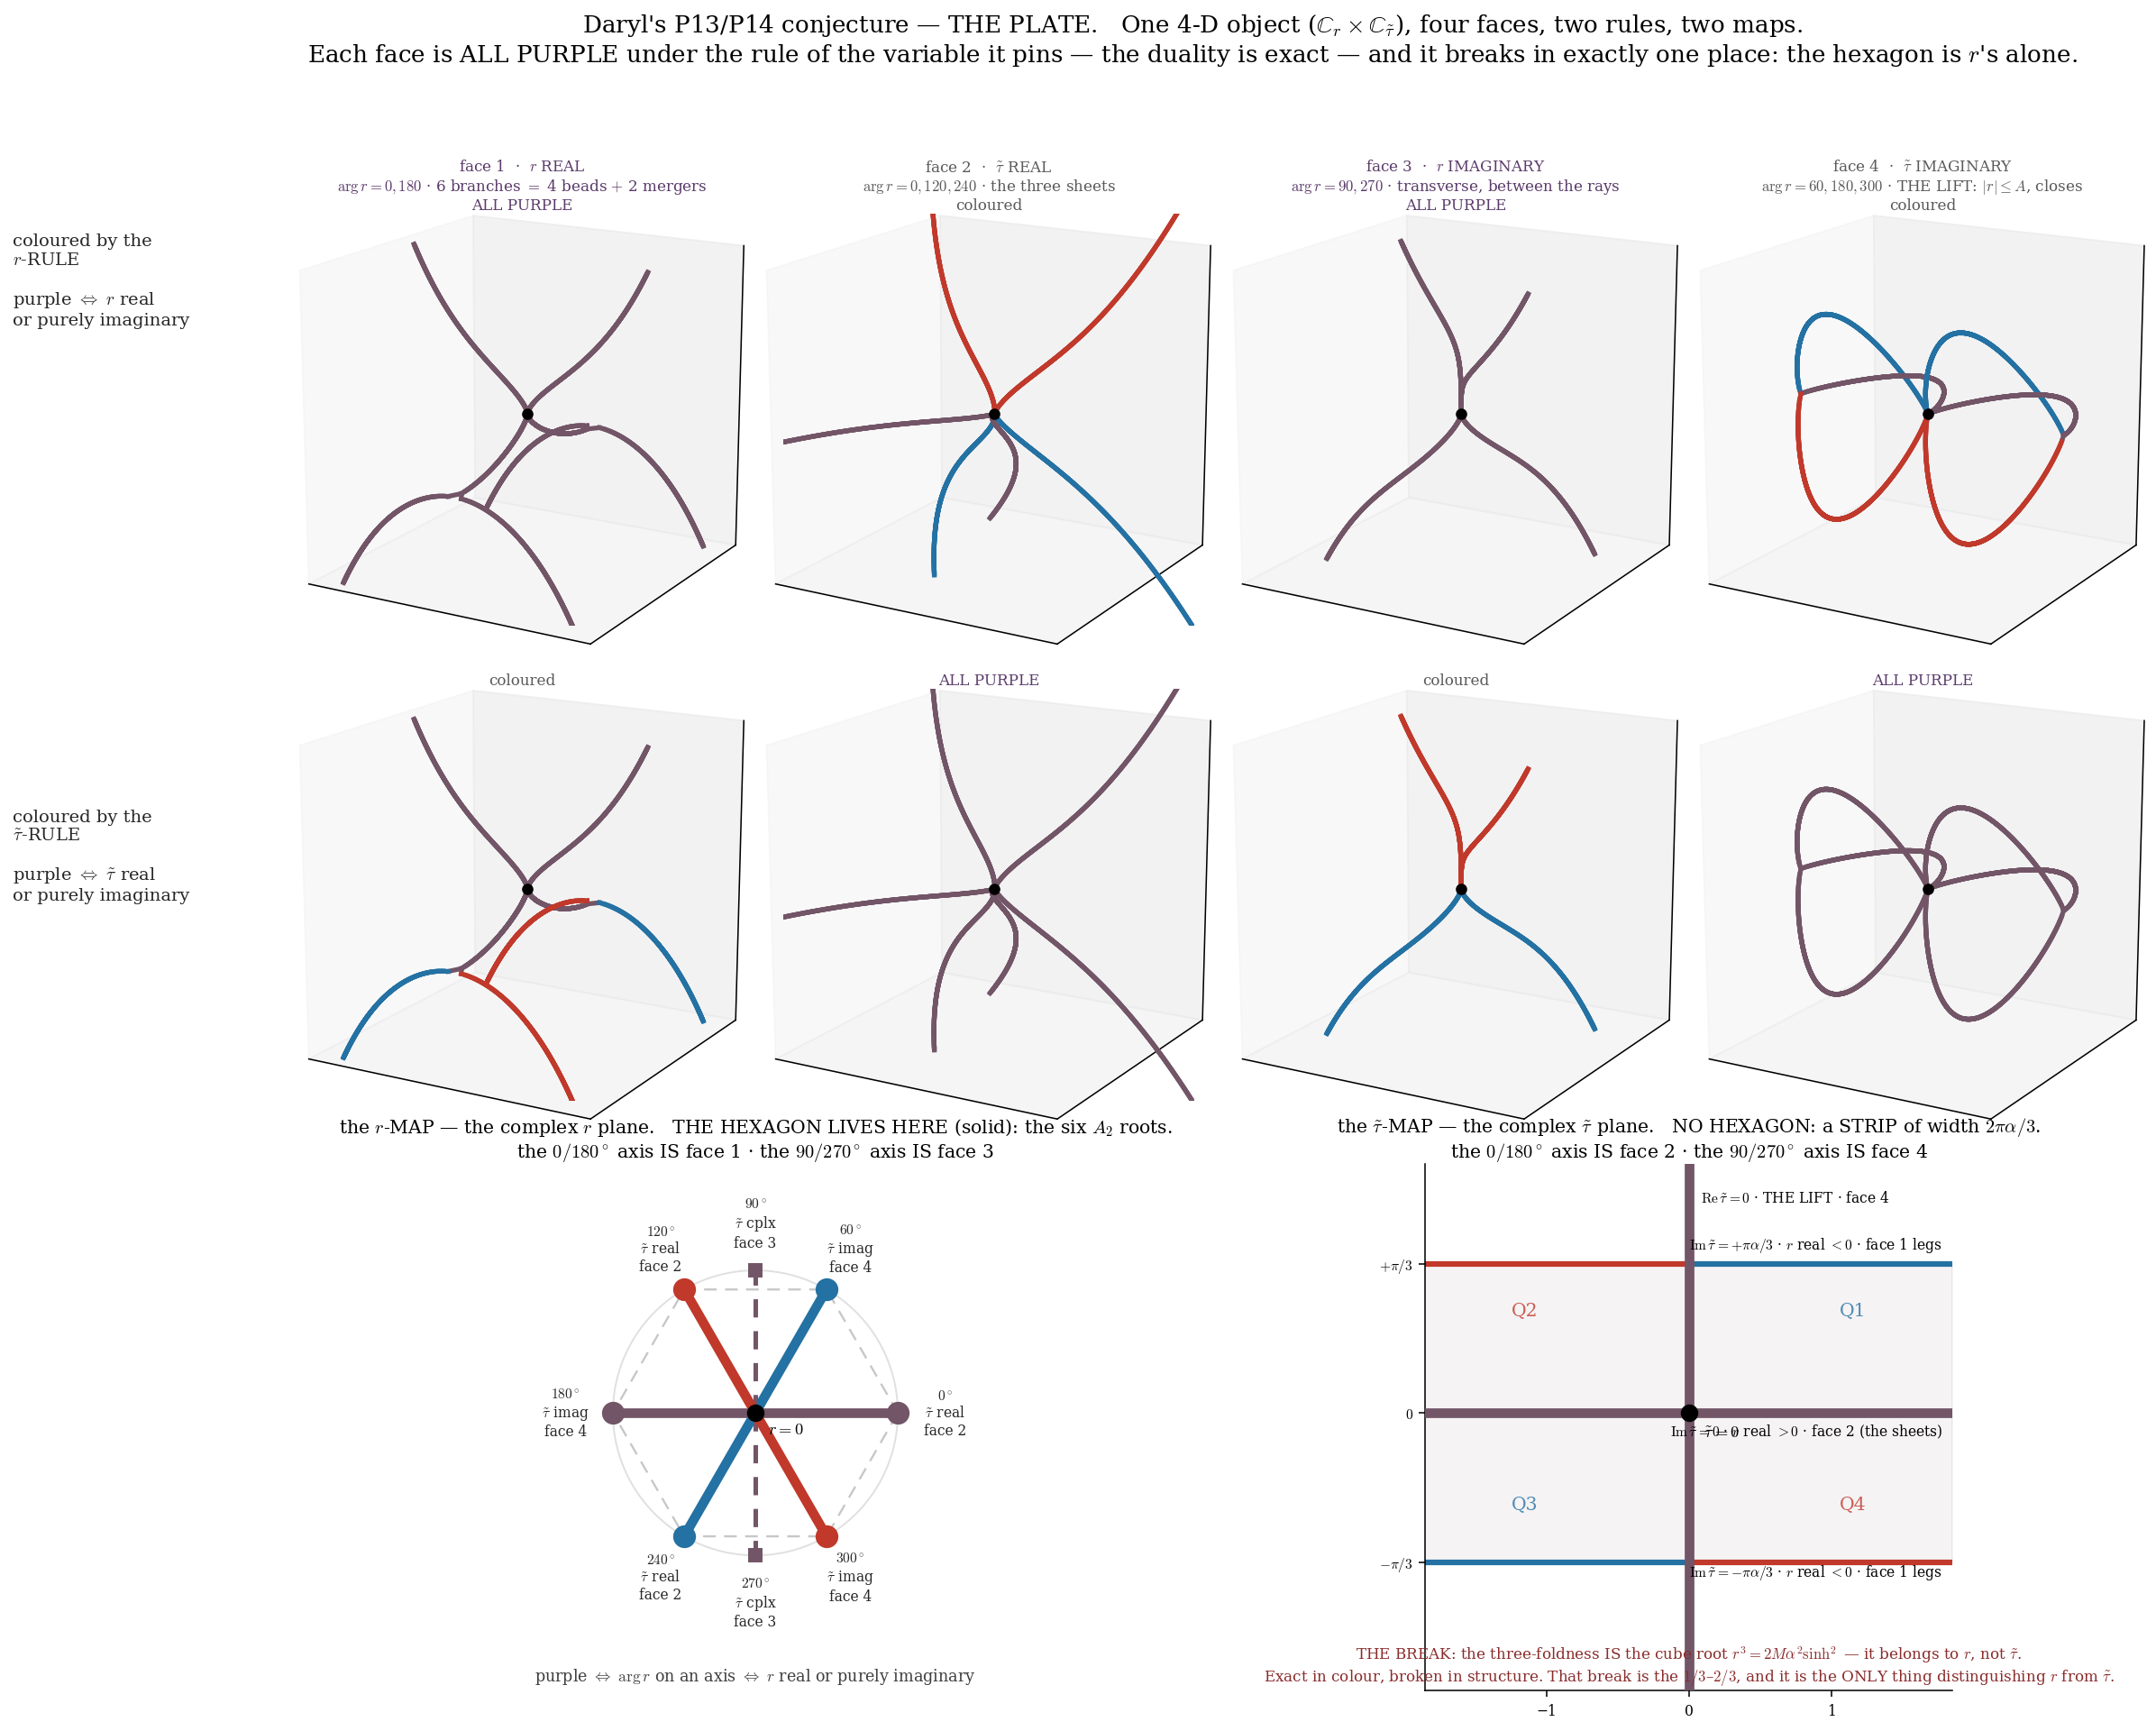
\includegraphics[width=\textwidth]{daryl_p13p14_THE_PLATE.png}
\caption{\textbf{The Plate: the full analytic object $\mathbb{C}_r\times\mathbb{C}_{\tilde\tau}$ on which the closure is stated (figure draft, to be finalised).} The cosmogenetic bead $r^{3}=2M\alpha^{2}\sinh^{2}(3\tilde\tau/2\alpha)$ drawn as its four faces---the $2\times2$ of $\{r,\tilde\tau\}\times\{\text{real},\text{imaginary}\}$---under the two colouring rules and the two coordinate maps. The $r$-axis carries the $A_2$ hexagon, the discrete residue read as the three roots (the matter sector's flavour skeleton~\cite{JanzenMatter}); the $\tilde\tau$-axis carries the cosmogenetic lap, the two conjugate wings meeting at the branch point $r=0$. The mass-reflection $R$ and the reality involution $K$ of Proposition~\ref{prop:conjugation-closure} are the two axis-symmetries of this one object, and the real slice ($r,\tilde\tau$ real) is the cosmological hyperboloid the framework paper draws panel by panel~\cite{JanzenCRframework}. The conjugation of charge and the discrete residue of matter are thus one structure read two ways---Daryl's $P13/P14$ conjecture, carried here and drawn in full at the matter-sector seam.}
\label{fig:the-plate}
\end{figure}

The scope is stated as sharply as the boundary. What is established is a factorisation of $C$ at the level of the bead geometry: its kinematic content is geometric, its charge sign field-level. What is \emph{not} established here, and is established in the matter sector~\cite{JanzenMatter}: that the geometric involution $R\circ K$ acts on the built fermion sector's zero-modes as the field-theoretic $C$---the matter-sector paper takes this up and confirms the \emph{kinematic} face on the actual zero-modes ($R$ carrying each generation to its bound antimatter partner on the reversed wall, the seam continuation supplying $K$), the full antilinear $C$ with its charge still closing from the field~\cite{JanzenMatter}; that a wing of the bead is a \emph{specific} charged particle (the identification needs the charge the geometry does not source, and the world-correspondence the data judge); or that a geometric $CPT$ is thereby auto-yielded (it is not---the charge still closes from the field). Nor does the factorisation vindicate a ``species $=\operatorname{sign} r$'' reading: the maps are stated on the full object, where $\operatorname{sign} r$ has no meaning off the real axis, and the particle/antiparticle content is the Feynman--St\"uckelberg relation the object carries, not the slice's sign. What Proposition~\ref{prop:conjugation-closure} settles is the boundary's inside at exactly the earned weight: the geometry carries $C$'s kinematics, the field carries $C$'s charge, and the seam between them is the cosmogenesis.

\begin{proposition}[The residue is the cosmogenesis's own symmetry]\label{prop:residue-is-the-bead}
The factorisation above says what $C$ breaks into. This says what the residue \emph{is}, and the two are not the same statement. The discrete residue the wall leaves is not an inert remainder the substrate happens to carry alongside its cosmology: \emph{it is the cosmogenetic bead's own symmetry.} The orientation parity $R$ is the single reflection $r\mapsto-r$, and that one map simultaneously
\begin{enumerate}
\item[\textup{(i)}] carries the fundamental to the antifundamental, $\bar{\mathbf 3}=R(\mathbf 3)$---the matter/antimatter skeleton;
\item[\textup{(ii)}] reverses the mass, $2M\mapsto-2M$;
\item[\textup{(iii)}] swaps the substrate's two null rulings---though this face, alone among the four, is \emph{generic}: \emph{every} orientation-reversing isometry swaps them, so it distinguishes nothing and nothing below leans on it; and
\item[\textup{(iv)}] \textbf{fixes exactly the locus $r=0$, which is the bead's branch point}, and exchanges the two signed-radius regions the bead's halves occupy~\cite{JanzenCRframework}.
\end{enumerate}
\emph{One $\mathbb{Z}_2$, four faces.} The content is \textup{(i)} with \textup{(iv)}: \textbf{the conjugation's fixed point is the cosmogenesis's branch point.} The bead passes \emph{through} the one locus $R$ fixes, and in doing so passes from the region $R$ labels $\mathbf 3$ to the region it labels $\bar{\mathbf 3}$.
\end{proposition}

\begin{proof}
\textup{(i)}--\textup{(iii)} are the companion algebroid and groupoid constructions: $R=\mathrm{diag}(1,1,-1,1,1,1)\in\mathrm{O}(5,1)\setminus\mathrm{SO}_0(5,1)$ is a substrate isometry of determinant $-1$ globally and on the ruled three-block, which swaps the two rulings and, $2M=r_0-r_0^3$ being odd, sends $2M\mapsto-2M$; it is the $A_2$ diagram automorphism, hence $\mathbf 3\leftrightarrow\bar{\mathbf 3}$---and that step, which reads as though negating the roots were generally the same as conjugating the representation, holds for a reason peculiar to $A_2$ and worth stating: $-1\notin W(A_2)$, so negation is \emph{outer}, and since $\mathrm{Aut}(A_2)/W$ has order two it and the diagram automorphism lie in the one non-trivial coset and generate the same $\mathbb{Z}_2$. In a system where $-1$ \emph{is} Weyl---$A_1$, $B_2$, $G_2$, every rank-two system but this one---negation would be inner and would conjugate nothing. For \textup{(iv)}: $R$ is an involution, so its fixed set is $\{r:r=-r\}=\{0\}$, and $r=0$ is the branch point through which the bead's signed slicing continues onto the conjugate branch; since species is the region label $\operatorname{sign}r$ and $R$ exchanges the regions bijectively, the bead's two halves carry conjugate species. \emph{(Receipts: \rcpt{P13_closure_i_check}, \rcpt{P13_closure_iv_check}, \rcpt{P13_ruling_swaps}.)}
\end{proof}

\begin{remark}[The asymmetry is the content, not a blemish on it]\label{rem:closure-asym}
Proposition~\ref{prop:residue-is-the-bead} claims a \emph{co-location}---one map's fixed point is the other's branch point---and pointedly not that $R$ carries one leg of the bead onto the other. It does not, and the distinction is load-bearing. $R$ is a reflection; the bead's passage through $r=0$ is a continuation; \emph{a map is not a path}. And the two legs are \emph{not} mirror images: read in cosmic time the collapse leg goes as $\cosh^{2/3}$ and the expansion leg as $\sinh^{2/3}$, so they are structurally distinct curves---as the framework's own figure states, \emph{``a run and a lift against a single real curve, not mirrors''}~\cite{JanzenCRframework}.

That the bead is \emph{not} $R$-symmetric is no defect in the correspondence; it is what makes the crossing an \emph{event}. Were the legs mirrors, the bead would be invariant under the very reflection whose regions label its species, and there would be no asymmetry for the cosmogenesis to carry. Species is a region label and needs only that $R$ exchange the regions; the curve's shape is free to be asymmetric, and is. \emph{The asymmetry is the conjugation's content, not a footnote to it.}
\end{remark}

\paragraph{What the two closures say together.} The factorisation fixes \emph{what $C$ is made of}; Proposition~\ref{prop:residue-is-the-bead} fixes \emph{what the geometric factor is}---and it is not a fragment of machinery that happens to sit in the substrate, it is the symmetry of the object the cosmology \emph{is}. So the substrate's contribution to matter is not a separate gift standing beside its cosmology: \textbf{it is the cosmogenesis, read on its discrete structure instead of its continuous one.} The companion framework's antimatter-progenitor theorem is then this boundary's first consequence rather than an independent result---the progenitor collapse is antimatter relative to our expansion \emph{because} the bead's two halves lie in the regions the conjugation exchanges, on either side of the locus it fixes~\cite{JanzenCRframework}. And the matter-sector facts fall in as instances of one thing: that the generations \emph{originate} at the Nariai crest, that the crest is a fixed point of the family symmetry but \emph{not} of $R$, and that consequently no matter/antimatter asymmetry is a cosmogenesis event but a standing relation across the bead~\cite{JanzenMatter}.

This is what the negative boundary was always mapping. The wall's content is that the substrate cannot supply matter's \emph{content}; the closure's content is that what it \emph{does} supply is not a fragment but the cosmogenesis's own discrete structure---and that \textbf{the two questions the corpus keeps apart---what conjugates matter, and what became of the collapsed universe---are questions about one map.}

\section{The physics synthesis: the framework and the gauge as the substrate's two real forms}\label{sec:synthesis}

Section~\ref{sec:face-status} fixed the two real forms and the asymmetry between them; the closure of \S\ref{sec:closure} read the discrete structure they share. What remains is the continuous inside of the same boundary. It is not that the substrate yields the Standard Model---the wall stands, $\su(3)$ no Lorentzian isometry---but that the divide the last century drew \emph{between} the gravitational and the quantum, and between gravity and the gauge forces, is one substrate read on its two real forms. This is the positive result the two-real-forms structure was pointed at from the start, stated at the weight its pieces carry.

\paragraph{The Lorentzian form carries the framework.} The real form the matter rides is not merely where general relativity's solutions live; it is where general relativity's \emph{quantum framework} lives. The hypersurface-deformation (Dirac) constraint algebra that is the canonical root of the problem of time is the symmetric-space coset structure of the Lorentzian substrate $\SO(5,1)/\SO(4,1)$, its structure function the coset metric and the ``wrong sign'' that obstructs a global time the coset's own indefinite signature~\cite{JanzenAlgebroid}. Read on the empirically forced foliation the scalar constraint deparametrizes to a true Hamiltonian generating unitary advance in cosmic time, the frozen Wheeler--DeWitt constraint and that Hamiltonian the same content differing only in whether the manifold is granted existence~\cite{JanzenCanonicalTime}. So the framework's whole apparatus---the constraint algebra, the problem of time and its deparametrization cure, the unitary cosmic-time evolution, the discrete graviton tower that projects to the flat-$\Lambda$CDM mode---is carried by the Lorentzian real form, on the horn the matter rides and the cuts the flavour residue grades~\cite{JanzenMatter}. The temporal, existent physics is one real form's content.

\paragraph{The Euclidean form carries the gauge and the quantum scale.} The colour $\su(3)$ lives on the compact face reached by the global Wick alone---operation (3) of the seam, $S^{5}=\SO(6)/\SO(5)$, not the seam continuation's $S^{4}=\SO(5)$ (\S\ref{sec:setup},~\S\ref{sec:decoupling})---because colour requires the \emph{full} $\SO(6)$: the smallest faithful real representation of $\su(3)$ is six-dimensional (the $\mathbf 3\oplus\bar{\mathbf 3}$, realified antisymmetric), so $\su(3)\subset\so(6)$ but $\not\subset\so(5)$, and the Lorentzian compact sector supplies only five. The quantum of action enters through the de Sitter horizon's Gibbons--Hawking thermal state, a Euclidean continuation of period $\beta=2\pi\alpha$~\cite{JanzenCanonicalTime,JanzenGeometricCore}---and that Euclidean is the \emph{same} face. The thermal regularity's sphere is the global-Wick $S^{5}$ (its period independent of dimension, the round sphere its Euclidean section), and it cannot be stranded on a smaller carrier than the one $\su(3)$ already requires whole. So the quantum of action and the colour symmetry share the one Euclidean real form the way $c,\Lambda,G$ share the Lorentzian one---gauge on it because operation (3) is the only seam operation that lands there, $\hbar$ on it because the horizon's Euclidean is that same sphere (receipt \rcpt{P13_qm_S4_vs_S5}).

\begin{figure}[t]
\centering
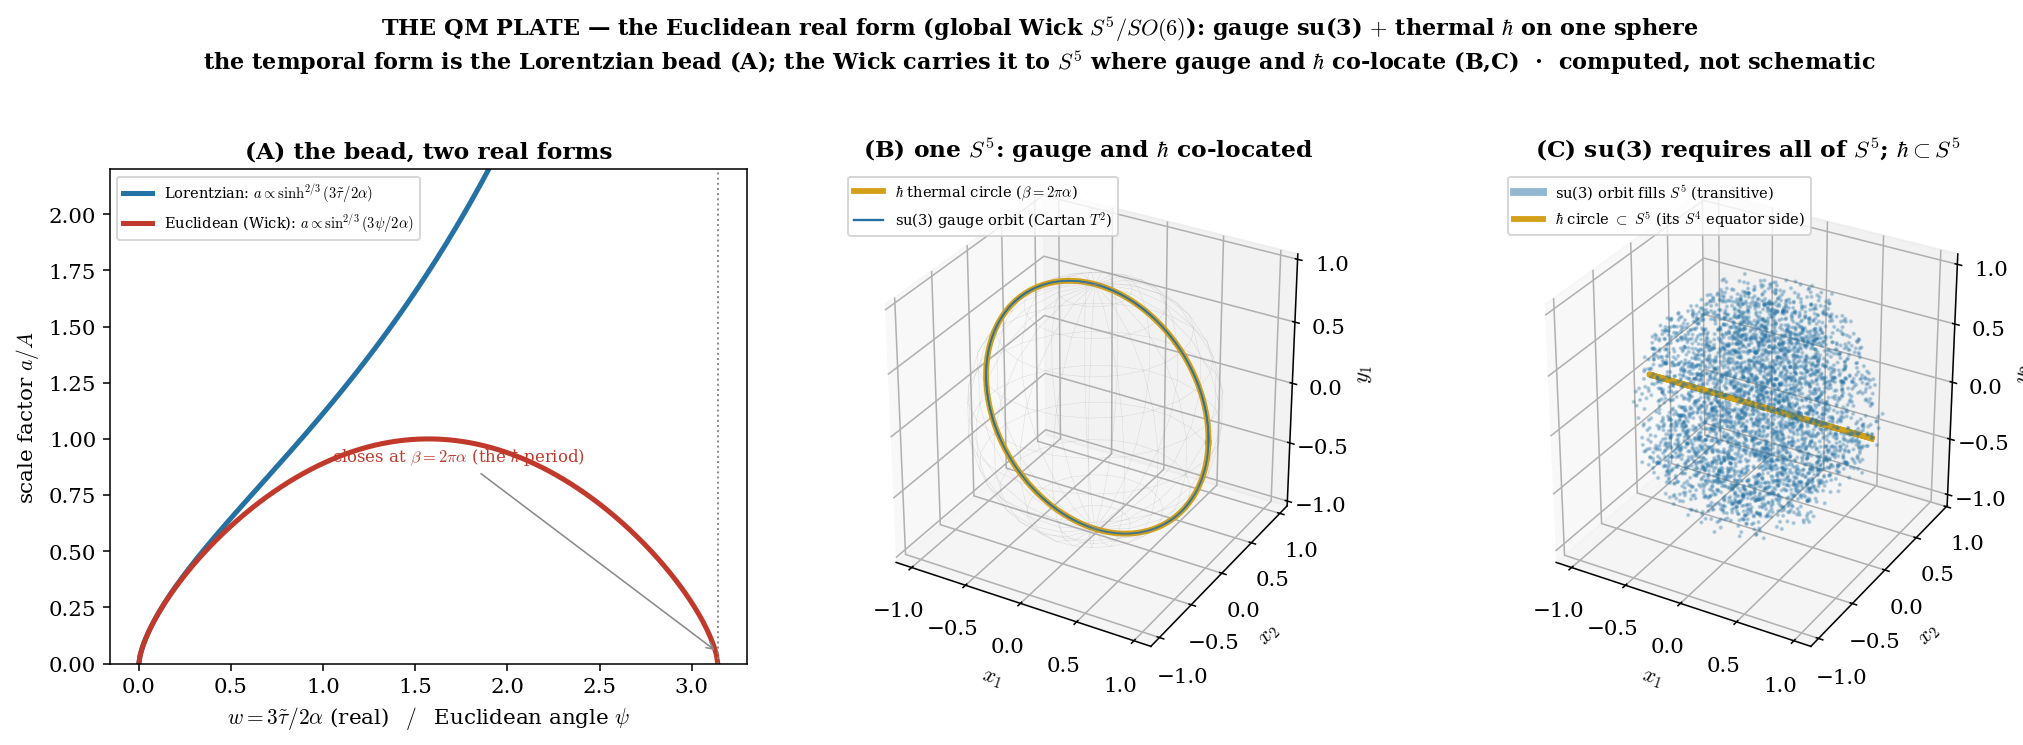
\includegraphics[width=\textwidth]{qm_central_figure.png}
\caption{\textbf{The QM Plate: the Euclidean real form, gauge and $\hbar$ on one sphere (figure draft, to be finalised).} The companion to Figure~\ref{fig:the-plate} on the substrate's \emph{other} real form. \textbf{(A)} the bead's two real forms as one analytic curve---the Lorentzian $\sinh^{2/3}$ (the open, temporal expansion) and its Euclidean Wick $\sin^{2/3}$, which closes at $\beta=2\pi\alpha$, the horizon's thermal period. \textbf{(B)} the global-Wick $S^{5}=\SO(6)/\SO(5)$ carrying a $\su(3)$ gauge orbit (a Cartan torus) and the $\hbar$ thermal great circle together, co-located on the one sphere. \textbf{(C)} a $\su(3)$ trajectory fills $S^{5}$ (the action is transitive) while the $\hbar$ circle is a sub-orbit---the drawn form of $\su(3)\subset\so(6)$, $\not\subset\so(5)$: gauge needs the whole sphere. All curves are integrated from the realified $\su(3)\subset\so(6)$ generators (receipt \rcpt{P13_qm_S4_vs_S5}); the projections of (B,C) are three-dimensional shadows of the five-sphere.}
\label{fig:qm-plate}
\end{figure}

\paragraph{The framework straddles; the quantum is not a third thing.} This locates ``the quantum'' precisely, and it is not a separate ingredient the geometry must also produce. The framework's \emph{structure}---the constraint algebra, unitarity, the discreteness of the graviton tower, the problem of time and its cure---is Lorentzian, the temporal real form's own. Only the framework's \emph{scale}, the quantum of action $\hbar$, is set on the Euclidean face, by the horizon's thermal state, which closes the free sector's lone quantization ambiguity without a free parameter~\cite{JanzenCanonicalTime}. So the quantum enters the corpus not as a fifth force awaiting geometrization but as the thermal gauge of the compact real form, its framework already carried by the Lorentzian one. The continuous dynamics is first-class general relativity, admitting rather than forcing a quantum structure, any forcing isolated to the discrete root structure and not the continuous evolution~\cite{JanzenAlgebroid,JanzenMatter}.

\paragraph{The synthesis.} Put together: the substrate wears two real forms of the one complex group $\SO(6,\mathbb{C})$, and each carries one side of the divides the corpus keeps apart. The Lorentzian form $\SO(5,1)$ is the existent temporal world---general relativity, the framework, the matter, the flavour the residue grades, and the classical cosmology whose fluctuations are inherited progenitor content rather than a substrate quantum vacuum~\cite{JanzenCRcosmology}. The Euclidean form $\SO(6)$ is the atemporal structure that world carries---the gauge group and the quantum scale together---real by construction but no co-equal existent, holding no clock (\S\ref{sec:face-status}). The two meet at the horizon where $\beta=2\pi\alpha$, the join already present in the complexification the substrate was reached through. On this reading the general-relativity/quantum divide and the gravity/gauge divide are not two unifications owed but one fact: one substrate, one complex group, read on its two real slices. The wall is not breached---the reading places $\su(3)$ exactly where the wall does, across the seam on the compact face---but what the wall encloses is now stated at the level of the real forms, not only the discrete residue. This is the continuous companion to \S\ref{sec:closure}: there, the substrate's discrete structure is the cosmogenesis read on its residue; here, its continuous structure is the framework and the gauge read on its two real forms.

\paragraph{What the synthesis dissolves.} Gathered, the two-real-forms reading is one dissolution seen twice, and of the same kind the framework paper performs on general relativity's pathologies~\cite{JanzenCRframework}---not a reconciliation engineered between two structures, but the recognition that the structures were one. Two of the last century's standing divides are its subjects. The \emph{gravity--gauge divide}---gravity and the Yang--Mills forces taken as separate structures awaiting unification---dissolves by identity: general relativity's solution space is the cuts of the Lorentzian real form $\SO(5,1)$, and the colour group is the $\su(3)\subset\so(6)$ the Euclidean real form $\SO(6)$ carries, the two being the real forms of the one complex $\SO(6,\mathbb{C})$---not two forces to join but one substrate read on its two slices. The \emph{general-relativity--quantum divide}---the incompatibility a quantum gravity is asked to repair---dissolves the same way: general relativity's quantum \emph{framework}, the constraint algebra and the problem of time, is already the Lorentzian form's own symmetric-space structure~\cite{JanzenAlgebroid,JanzenCanonicalTime}, and only the quantum \emph{scale} $\hbar$ is set on the Euclidean face by the horizon's thermal state, so the quantum is not a third thing to reconcile with gravity but the thermal gauge of gravity's own conjugate real form. The two are therefore not two unifications owed but one fact read twice---the consolidation the epistemic discipline reads as the signature of a sound framework~\cite{JanzenShadowExistence}: where the standard expectation meets each divide with a separate programme, this reading meets both with one substrate, \emph{requiring} the identity where a reconciliation would merely \emph{permit} one arrangement among many. The altitude is held with the paper's own care: the \emph{pieces} are established---the constraint algebra as the Lorentzian coset, colour's need of the full $\so(6)$ ($\su(3)\subset\so(6)$ but $\su(3)\not\subset\so(5)$, computed), and $\hbar$ on the same global-Wick $S^{5}$ the horizon's Euclidean closes on---while the \emph{world-correspondence}, that these real forms are physics' actual quantum and gauge sectors rather than a structural rhyme, stays the reach the synthesis asserts no further. The dissolution is thus by identity at the level of the structure and, at the level of the world, at the discipline's coherence and not its correspondence.

\paragraph{What it feeds.} The synthesis is what lets the cosmology close classically. Because the framework is Lorentzian and the quantum scale is only the compact face's thermal gauge, the existent cosmology is classical through and through: the acoustic and abundance data it must meet are met on the real horn, the graviton tower deparametrized and projected to the flat-$\Lambda$CDM mode without a free parameter, the quantum structure walled to the Euclidean face it never leaves~\cite{JanzenCRcosmology,JanzenCosmogenesis}. The cosmogenesis paper's matter history and the cosmology paper's rate and abundances are computed on the one real form, with the gauge and the quantum of action located---not omitted---on the other. The physics synthesis feeds the cosmological closure precisely by keeping the quantum where the two real forms put it.

\textbf{[The pieces are established: the constraint algebra as the Lorentzian coset and its deparametrization~\cite{JanzenAlgebroid,JanzenCanonicalTime}, colour on the compact face and its ontological status (\S\ref{sec:decoupling},~\S\ref{sec:face-status}), the horizon's thermal gauge~\cite{JanzenGeometricCore}. The $\su(3)\subset\so(6)$, $\not\subset\so(5)$ co-location of the gauge and thermal Euclideans on the one $S^{5}$ is computed (\rcpt{P13_qm_S4_vs_S5}). Reading the two real forms as carrying the framework and the gauge is the synthesis this paper draws, its geometric closure recorded at the core~\cite{JanzenGeometricCore}. The world-correspondence---that these real forms are the actual quantum and gauge sectors of physics rather than a structural rhyme with them---is the interpretive reach the corpus holds open, drawn here at exactly that weight and asserted no further.]}

\section{What it means for the programme}\label{sec:meaning}

The boundary is not a setback to CR's gravitational claim; it sharpens it. The substrate is the complete gravitational object---$\dS_5$ has no continuous symmetry beyond $\SO(5,1)$, and the slicing operator generates the gravitational solution space from it---and the present result says, precisely, that this completeness does \emph{not} extend to the matter sector through isometry. That exhaustion is one face of the substrate's maximal symmetry read across the corpus~\cite{JanzenGeometricCore}: the same completeness that locks the cosmological constants and fixes the parameter-free rate is what walls a continuous geometric colour, the wall its matter-boundary face and the discrete orientation parity $\mathrm{O}(5,1)\setminus\mathrm{SO}_0$ the leading residue it leaves---enlarged in \S\ref{sec:closure} to carry, together with the antilinear complex-analytic face, charge conjugation's kinematic content (do-not-assert the fermion realisation). What positive structure that discrete residue may carry---the full automorphism $\mathrm{Aut}(A_2)=S_3\times\mathbb{Z}_2\cong D_6$ read on a fermion sector as three generations times two chiralities, and with it a reading of the Standard Model's own discrete structure as a maximally-symmetric breaking of this maximally-symmetric substrate---is developed, as the conjecture it is and asserted nowhere as more, in the geometric-core paper~\cite{JanzenGeometricCore}, whose $A_2$ skeleton the slicing paper realises geometrically as a skew hexagon of null rulings~\cite{JanzenSlicing}; the present paper fixes only the perimeter within which any such reach must live. CR is then a gravitational-cosmological unification: one substrate, all the spherically symmetric stationary geometries, the dynamics up to the radiative wall. And on its two real forms it reaches further than that phrase alone conveys. The wall that places colour off the Lorentzian isometry is the same six-dimensional fact ($\su(3)\subset\so(6)$ but $\su(3)\not\subset\so(5)$) that places it, together with the quantum of action, on the substrate's Euclidean real form; and the constraint algebra that is general relativity's quantum framework is the Lorentzian real form's own (\S\ref{sec:synthesis}). What CR declines is the geometric unification of matter \emph{from isometry}; what it draws, on the substrate's two real forms, is the synthesis of \S\ref{sec:synthesis}---its wall intact, its world-correspondence held open.

There is a service in mapping a wall well. The geometric-unification programme has not obtained chiral generations from isometry, and the obstruction to it has stood since 1970; a precise statement of where and why the de Sitter substrate meets that same wall---grounded in the literature the gravitational corpus did not need to cite---spares the programme, and others, the cost of re-walking a road that three converging obstructions close. The bounded negative is itself a result: it is the honest perimeter of what one maximally symmetric Lorentzian substrate's geometry forces. And a perimeter drawn well encloses more than it excludes. What \S\ref{sec:closure} and \S\ref{sec:synthesis} state is the boundary's inside: on the substrate's discrete structure, charge conjugation's kinematic face is geometric, carried by the cosmogenesis bead's own $r=0$ crossing, with only the electric-charge sign closing from the field; and on its continuous structure, the two real forms carry the quantum framework and the gauge---one substrate read on its two slices, the general-relativity/quantum and gravity/gauge divides on that reading a single fact. These are the positive results the negative alone could not reach, and a drawn connection between charge conjugation, the quantum framework, and the cosmology. The paper that began by mapping a family of negative boundary results thereby closes them into a shape, and draws the shape's inside.

\begin{thebibliography}{9}
\bibitem{JanzenThesis} D.~Janzen, \emph{A Solution to the Cosmological
Problem of Relativity Theory} (PhD dissertation, University of Saskatchewan,
2012), ch.~3.
\bibitem{PeskinSchroeder} M.~E. Peskin and D.~V. Schroeder, \emph{An Introduction to Quantum Field Theory}, Addison--Wesley (1995), \S3.4 (charge conjugation: the matrix $C=\mathrm{i}\gamma^{2}\gamma^{0}$ and the field map $\psi^{c}=C\bar\psi^{\top}$).
\bibitem{JanzenCircle} D.~Janzen,
\emph{The Schwarzschild and de Sitter circle: the intrinsic geometry of one homogeneous ring---the event horizon and the curvature singularity at $r=0$ its two poles}, companion paper (P2).
\bibitem{JanzenOperator} D.~Janzen, \emph{Covariance of geometries over the de Sitter substrate: the slicing operator, the vacuum kernel, and matter as the bend of the cut}, companion paper (P8).
\bibitem{JanzenRange} D.~Janzen, \emph{The range of the de Sitter slicing operator: surjectivity onto the symmetry-reducible sector of general relativity, the Kerr--NUT--(A)dS vacuum kernel, and the wall of inhomogeneity}, companion paper (P9).
\bibitem{JanzenBHcausality} D.~Janzen, \emph{The event horizon is a metric singularity: a missing definition in general relativity}, companion paper (P1).
\bibitem{JanzenCRframework} D.~Janzen, \emph{Collapsed matter must become a universe: the necessary and sufficient augmentation of general relativity into a description of structural existence, proven for gravitational collapse of any symmetry}, companion paper (P7).

\bibitem{JanzenCanonicalTime} D.~Janzen, \emph{The canonical problem of time as a category error: an empirically forced cosmic time, deparametrization, the dissolution of frozen dynamics, and a graviton quantization the de~Sitter horizon closes without a free parameter---the seam where $\hbar$ enters gravity---in Cosmological Relativity}, companion paper (P10).
\bibitem{JanzenModernParallax} D.~Janzen, \emph{The modern parallax: the redshift-isotropy floor, the empirical forcing of cosmic time and uniform expansion, and the measured resolution of the relativity of simultaneity}, companion paper (P4).
\bibitem{JanzenShadowExistence} D.~Janzen, \emph{The shadow of existence: scientific theory-choice as an empirically grounded discipline, calibrated on the historical record}, companion paper (P6).
\bibitem{JanzenDynamics} D.~Janzen, \emph{Why the cut bends: the dynamics of the de Sitter cut, the confined gravitational wave, the generative boundary of the slicing operator, and chirality as the turning of the polarization plane}, companion paper (P11).
\bibitem{JanzenAlgebroid} D.~Janzen, \emph{General relativity's constraint algebra as the symmetric-space structure of a de Sitter substrate: the action Lie algebroid of the symmetry-reducible sector, and the problem of time's ``wrong sign'' as the substrate's coset signature}, companion paper (P12).
\bibitem{JanzenGeometricCore} D.~Janzen, \emph{Reached through the imaginary, real by construction: the maximally symmetric substrate as the geometric--ontological core}, companion paper (p0).
\bibitem{Witten1981} E.~Witten, \emph{Search for a realistic Kaluza--Klein theory}, Nucl.\ Phys.\ B \textbf{186} (1981) 412.
\bibitem{Witten1983} E.~Witten, \emph{Fermion quantum numbers in Kaluza--Klein theory}, in \emph{Shelter Island II: Proceedings of the 1983 Shelter Island Conference on Quantum Field Theory and the Fundamental Problems of Physics}, eds.\ R.~Jackiw, N.~Khuri, S.~Weinberg, E.~Witten (MIT Press, 1985) 227.
\bibitem{AtiyahHirzebruch1970} M.~F.~Atiyah and F.~Hirzebruch, \emph{Spin-manifolds and group actions}, in \emph{Essays on Topology and Related Topics} (Springer, 1970) 18.
\bibitem{LawsonYau} H.~B.~Lawson and S.~T.~Yau, \emph{Scalar curvature, non-abelian group actions, and the degree of symmetry of exotic spheres}, Comment.\ Math.\ Helv.\ \textbf{49} (1974) 232.
\bibitem{JanzenSlicing} D.~Janzen, \emph{The de Sitter substrate and its slicing curve: horizons as turning points, and de Sitter and Schwarzschild as two readings of one slicing}, companion paper (P3).
\bibitem{JanzenGroupoid} D.~Janzen, \emph{The Schwarzschild--de Sitter description groupoid: generators, relations, and Schwarzschild as the asymmetric realisation}, companion paper (P5).
\bibitem{JanzenMatter} D.~Janzen, \emph{The fermion sector of Cosmological Relativity: three chiral generations from the maximally-symmetric slicing structure}, companion paper (P14).
\bibitem{JanzenCosmogenesis} D.~Janzen, \emph{Cosmogenesis: the Big Bang as a synthesis of Cosmological Relativity's deductively forced consequences, and the primordial light-element abundances it produces}, companion paper (P16).
\bibitem{JanzenCRcosmology} D.~Janzen, \emph{The cosmology of Cosmological Relativity: the expansion history from causal reassignment on a de~Sitter background, the cosmogenesis branch point, and the scalar perturbation sector}, companion paper (P15).
\bibitem{GeorgiGlashow1974} H.~Georgi and S.~L.~Glashow, \emph{Unity of all elementary-particle forces}, Phys.\ Rev.\ Lett.\ \textbf{32} (1974) 438.
\bibitem{FritzschMinkowski1975} H.~Fritzsch and P.~Minkowski, \emph{Unified interactions of leptons and hadrons}, Ann.\ Phys.\ (N.Y.) \textbf{93} (1975) 193.
\bibitem{AtiyahSinger1968} M.~F.~Atiyah and I.~M.~Singer, \emph{The index of elliptic operators.\ I}, Ann.\ of Math.\ \textbf{87} (1968) 484.
\bibitem{Lichnerowicz1963} A.~Lichnerowicz, \emph{Spineurs harmoniques}, C.\ R.\ Acad.\ Sci.\ Paris \textbf{257} (1963) 7.
\bibitem{LawsonMichelsohn1989} H.~B.~Lawson and M.-L.~Michelsohn, \emph{Spin Geometry} (Princeton University Press, Princeton, 1989).
\end{thebibliography}


\clearpage
\section*{Appendix R\quad Computational Receipts}\label{app:receipts}
\addcontentsline{toc}{section}{Appendix R: Computational Receipts}
\small\noindent Each computation marked \rcptmarker\ in the text is verified by a runnable receipt in the \texttt{receipts/} directory that ships with this work; status \textsf{OK} = verified (traced, run, output matches the claim). This appendix is generated from the receipt index, not maintained by hand.\par\medskip
\begingroup\renewcommand{\arraystretch}{1.25}
\begin{description}
\item[\label{rcpt:P13_A3_factorization}\texttt{P13\_A3\_factorization}]\hfill\textsf{[OK]}\\
\textit{prop:conjugation-closure} \ (charge conjugation factorises on the bead: C=(Q->-Q)\_field o (R o K)\_geometric; R o K is antilinear geometric involution reproducing C's kinematic (CPT/FS) content but BLIND to sign(Q) (Q enters as Q\textasciicircum{}2)). 
\emph{Computes:} numeric on random complex points: R,K,C on bead; \textbar{}mass\textbar{}/species/FS-wings; load-bearing NEGATIVE R o K blind to Q sign
 \emph{Bound:} scope + do-not-assert stated
\ \emph{Run:} \texttt{python3 receipts/P13\_boundary\_paper/P13\_A3\_factorization.py}
\item[\label{rcpt:P13_conjugation_parity}\texttt{P13\_conjugation\_parity}]\hfill\textsf{[OK]}\\
\textit{prop:conjugation-parity} \ (mass-reflection R=gamma\textasciicircum{}5 (grades chirality); mass term ODD, charge EVEN under r->-r; P=g1g2g3 flips chirality; R!=P (same residue, opposite parity-faces)). 
\emph{Computes:} cold read: parity of f(r) terms; Clifford R=g5 commutes / P anticommutes with g5; guards R!=P
\ \emph{Run:} \texttt{python3 receipts/P13\_boundary\_paper/P13\_conjugation\_parity.py}
\item[\label{rcpt:P13_ruling_swaps}\texttt{P13\_ruling\_swaps}]\hfill\textsf{[OK]}\\
\textit{prop:closure(iii)} \ (R swaps the substrate's two null rulings -- generic (every orientation-reversing isometry does)). 
\emph{Computes:} ruling swap under R; generic face
\ \emph{Run:} \texttt{python3 receipts/P13\_boundary\_paper/P13\_ruling\_swaps.py}
\item[\label{rcpt:P13_closure_i_check}\texttt{P13\_closure\_i\_check}]\hfill\textsf{[OK]}\\
\textit{prop:closure(i)} \ (R carries 3->3bar (matter/antimatter): (a) R negates roots => (b) A2 diagram automorphism => (c) 3<->3bar; A2-specific (warrant -1 not in W(A2))). 
\emph{Computes:} 3-link chain confirmed; flags the owed A2-specificity clause
 \emph{Bound:} corpus owed one clause
\ \emph{Run:} \texttt{python3 receipts/P13\_boundary\_paper/P13\_closure\_i\_check.py}
\item[\label{rcpt:P13_closure_iv_check}\texttt{P13\_closure\_iv\_check}]\hfill\textsf{[OK]}\\
\textit{prop:closure(iv)} \ (R:r->-r involution, fixed set \{r=0\} = the bead's branch point; two halves in R-conjugate regions; cosh/sinh asymmetry = the symmetry-breaking). 
\emph{Computes:} fixed point r=0 computed; corrects map-vs-path; asymmetry is content
\ \emph{Run:} \texttt{python3 receipts/P13\_boundary\_paper/P13\_closure\_iv\_check.py}
\item[\label{rcpt:P13_A3_spinor_lift}\texttt{P13\_A3\_spinor\_lift}]\hfill\textsf{[OK]}\\
\textit{prop:conjugation-parity (spinor)} \ (R o K lifted to the cut spinor IS charge conjugation: gamma\textasciicircum{}5 S psi*=-psi\textasciicircum{}c on 200 spinors; C=i g2 g0 the C-matrix proper; guard -i g2 is NOT C). 
\emph{Computes:} Clifford: g5 involution, reality-lift S unique, g5 S=-(C g0T), particle<->anti, Q\textasciicircum{}2 R-even; load-bearing C-matrix guard
\ \emph{Run:} \texttt{python3 receipts/P13\_boundary\_paper/P13\_A3\_spinor\_lift.py}
\item[\label{rcpt:P13_kretschmann_bead}\texttt{P13\_kretschmann\_bead}]\hfill\textsf{[OK]}\\
\textit{(bead Kretschmann)} \ (Kretschmann along the bead: mass CANCELS -- K=(12/alpha\textasciicircum{}4)(sinh\textasciicircum{}\{-4\}(3tau\textasciitilde{}/2alpha)+2), M-independent). 
\emph{Computes:} SdS K, bead r\textasciicircum{}3=2M a\textasciicircum{}2 sinh\textasciicircum{}2 w => r\textasciicircum{}6 kills M; numeric across 3 M values same K
\ \emph{Run:} \texttt{python3 receipts/P13\_boundary\_paper/P13\_kretschmann\_bead.py}
\item[\label{rcpt:P13_qm_S4_vs_S5}\texttt{P13\_qm\_S4\_vs\_S5}]\hfill\textsf{[OK]}\\
\textit{sec:synthesis} \ (Euclidean form carries gauge + hbar: su(3) subset so(6)/S\textasciicircum{}5 (faithful on R\textasciicircum{}6, not so(5)/S\textasciicircum{}4); GH beta=2pi alpha; S\textasciicircum{}4 subset S\textasciicircum{}5 equator => gauge and hbar SAME real form). 
\emph{Computes:} su(3) antisymmetry+faithfulness; dS\_n GH temp; S\textasciicircum{}4/S\textasciicircum{}5 nesting; verdict full-S\textasciicircum{}5 vs S\textasciicircum{}4-equator residue
\ \emph{Run:} \texttt{python3 receipts/P13\_boundary\_paper/P13\_qm\_S4\_vs\_S5.py}
\item[\label{rcpt:P13_cascade_rank}\texttt{P13\_cascade\_rank}]\hfill\textsf{[OK]}\\
\textit{sec:cascade} \ (cascade rank-map: rank(SM)=4 > rank SO(6)=3, so the full SM gauge group cannot embed even in the dS\_6 raise -- gauge structure dropped at the real cut). 
\emph{Computes:} so(6) Cartan (M12,M34,M56 commute, rank 3); su(3) rank 2; 4>3; SU(3)-fits control
 \emph{Bound:} supports prop:boundary
\ \emph{Run:} \texttt{python3 receipts/P13\_boundary\_paper/P13\_cascade\_rank.py}
\item[\label{rcpt:P13_sigma_lift}\texttt{P13\_sigma\_lift}]\hfill\textsf{[OK]}\\
\textit{sec:sigma} \ (a real involution is not the Wick rotation: sigma (real Weyl(A2) reflection) preserves eta\_L (in O(5,1)), the Wick x0->ix0 sends eta\_L->eta\_E; boost M05 -> rotation under Wick (so(6) created) but stays boost under sigma; su(3) faithful on R\textasciicircum{}6 (not so(5)) -- colour-from-geometry via sigma-lift does NOT hold). 
\emph{Computes:} Wick eta\_L->eta\_E; sigma preserves both signatures; boost->rotation vs boost->boost; su(3) faithful on R\textasciicircum{}6
 \emph{Bound:} bounded NEGATIVE, do-not-assert stated
\ \emph{Run:} \texttt{python3 receipts/P13\_boundary\_paper/P13\_sigma\_lift.py}
\item[\label{rcpt:L212_the_factorisation_singles_out_nothing}\texttt{L212\_the\_factorisation\_singles\_out\_nothing}]\hfill\textsf{[OK]}\\
\textit{sec:open} \ (the horizon cubic factorisation singles out no root). 
\emph{Computes:} every root satisfies 2M=r-r\textasciicircum{}3, so any root serves as r0; four values of 2M, all three roots each (14)
 \emph{Bound:} NOT-A-PAPER-CLAIM --- discharges L-212 move 1
\ \emph{Run:} \texttt{python3 receipts/P13\_boundary/L212\_the\_factorisation\_singles\_out\_nothing.py}
\item[\label{rcpt:Y1_supplying_the_requirement_made_it_an_ADD}\texttt{Y1\_supplying\_the\_requirement\_made\_it\_an\_ADD}]\hfill\textsf{[OK]}\\
\textit{sec:face-status} \ (supplying the DELETE reading's own precondition made the argument an ADD). 
\emph{Computes:} asserts the four real forms and the maximal-compact exclusion, and that P13 denies existence by a stated criterion rather than arbitrariness (14 checks)
 \emph{Bound:} NOT-A-PAPER-CLAIM --- discharges L-213
\ \emph{Run:} \texttt{python3 receipts/L213\_external\_constraint/Y1\_supplying\_the\_requirement\_made\_it\_an\_ADD.py}
\item[\label{rcpt:A1_the_venue_question_dissolves_and_curvature_remains}\texttt{A1\_the\_venue\_question\_dissolves\_and\_curvature\_remains}]\hfill\textsf{[OK]}\\
\textit{sec:frontiers} \ (the venue question for colour dissolves across three papers; what remains is curvature, because the built bundle is flat). 
\emph{Computes:} asserts the adjacent gap P13 advertises, the route P14 already built, and the flatness that relocates the question (13 checks)
 \emph{Bound:} NOT-A-PAPER-CLAIM --- L-211 run on L-213
\ \emph{Run:} \texttt{python3 receipts/L211\_closure\_adjacency/A1\_the\_venue\_question\_dissolves\_and\_curvature\_remains.py}
\item[\label{rcpt:P7_the_temperature_is_taken_and_the_entropy_never_is}\texttt{P7\_the\_temperature\_is\_taken\_and\_the\_entropy\_never\_is}]\hfill\textsf{[OK]}\\
\textit{sec:quantum} \ (R-P station 7: the corpus takes the de Sitter horizons TEMPERATURE as the channel through which the quantum of action enters, and never its ENTROPY --- and the entropy is where alpha and the Planck length meet). 
\emph{Computes:} counts the thermodynamic vocabulary against four zeros, asserts the black-hole decline and its scoping at source, matches beta=2pi alpha to r2527s kappa, and computes both quantities constant content (17 checks)
 \emph{Bound:} NOT-A-PAPER-CLAIM --- the finding is that it is UNASKED, not that it should be asserted
\ \emph{Run:} \texttt{python3 receipts/L204\_physics\_reach/P7\_the\_temperature\_is\_taken\_and\_the\_entropy\_never\_is.py}
\item[\label{rcpt:B2_the_mod_two_prerequisite_is_already_built}\texttt{B2\_the\_mod\_two\_prerequisite\_is\_already\_built}]\hfill\textsf{[OK]}\\
\textit{sec:conjugation} \ (PO-5 ranked \#1: the structure a mod-2 index needs is present, named, and REALISED ON THE BUILT ZERO-MODES --- R\ensuremath{\circ}K acts on the actual zero-modes as charge conjugations kinematic face). 
\emph{Computes:} counts the antilinear/reality material across the corpus, asserts P13s realisation sentence and P5s independent Z2-on-a-real-structure verbatim, and confirms the standard names are still at zero (13 checks)
 \emph{Bound:} NOT-A-PAPER-CLAIM --- establishes the prerequisite; no index computed or claimed to exist
\ \emph{Run:} \texttt{python3 receipts/L221\_the\_bridge/B2\_the\_mod\_two\_prerequisite\_is\_already\_built.py}
\item[\label{rcpt:B3_the_involution_is_quaternionic_not_real}\texttt{B3\_the\_involution\_is\_quaternionic\_not\_real}]\hfill\textsf{[OK]}\\
\textit{sec:conjugation} \ (PO-5s mod-2 route CLOSED: the antilinear involution is QUATERNIONIC --- the corpus own lift S=g0g1g3 squares to \ensuremath{-}1, so the index is valued in 2Z, not a parity). 
\emph{Computes:} asserts the lift verbatim, reproduces the corpus own identity g5S=\ensuremath{-}i g2 in Dirac and Weyl, verifies the Clifford algebra in both, and computes S\textsuperscript{2}=\ensuremath{-}1 (12 checks)
 \emph{Bound:} NOT-A-PAPER-CLAIM --- closes a route; the Kramers question it opens is untouched
\ \emph{Run:} \texttt{python3 receipts/L221\_the\_bridge/B3\_the\_involution\_is\_quaternionic\_not\_real.py}
\item[\label{rcpt:B7_two_unbuilt_sectors_not_one}\texttt{B7\_two\_unbuilt\_sectors\_not\_one}]\hfill\textsf{[OK]}\\
\textit{sec:open} \ (TWO unbuilt fermion sectors, not one: the Lorentzian PROPAGATING theory (PO-11) and the COMPACT-FACE gauge-acted sector, distinguished by boundary\_paper in one sentence and unbuilt for different reasons). 
\emph{Computes:} asserts the distinguishing clause, the remains-unbuilt clause, the no-equivariant-index clause and p0s propagating-sector wording verbatim, plus both reasons (7 checks)
 \emph{Bound:} NOT-A-PAPER-CLAIM --- corrects r2618s dedupe; table 27 to 28
\ \emph{Run:} \texttt{python3 receipts/L221\_the\_bridge/B7\_two\_unbuilt\_sectors\_not\_one.py}
\item[\label{rcpt:B61_the_walls_do_not_cover_the_spectral_route}\texttt{B61\_the\_walls\_do\_not\_cover\_the\_spectral\_route}]\hfill\textsf{[OK]}\\
\textit{sec:index} \ (THE INDEX OBSTRUCTIONS OWN HYPOTHESES DO NOT COVER THE SPECTRAL ROUTE: the boundary paper states them as "compactness and a continuous isometry", and inner fluctuations D -> D + A use NO isometry --- so the premise the paper says carries the theorem fails for it). 
\emph{Computes:} computes gamma\textasciicircum{}5 against the grading axioms, and pins the boundary papers own statement of the obstructions hypotheses and its known-escapes clause (5 checks)
 \emph{Bound:} NOT-A-PAPER-CLAIM --- the obstruction is sound within its hypotheses; two axioms (real structure J, order-one condition) remain untested and either can kill the route
\ \emph{Run:} \texttt{python3 receipts/L221\_the\_bridge/B61\_the\_walls\_do\_not\_cover\_the\_spectral\_route.py}
\item[\label{rcpt:C1_the_degree_six_dial_has_three_readings_and_the_paper_excludes_one}\texttt{C1\_the\_degree\_six\_dial\_has\_three\_readings\_and\_the\_paper\_excludes\_one}]\hfill\textsf{[OK]}\\
\textit{R-M station (C) / complex analysis, monodromy} \ (**THE \$Z\_6\$ DOES ACT, AND THE DEGREE-SIX DIAL HAS THREE READINGS, NOT TWO.** `M1` established that the equianharmonic \$Z\_6\$ and the monodromy \$S\_3\$ are same order and not isomorphic, and stated plainly that **"nothing here exhibits an action"**. It acts: \$D\_6=\textbackslash\{\}mathrm\{Aut\}(A\_2)\$ --- the corpus's own group, P13's --- has **exactly three** subgroups of order six, and the unique cyclic one is \$\textbackslash\{\}langle\$deck \$Z\_3\textbackslash\{\}rangle\textbackslash\{\}times\textbackslash\{\}langle\textbackslash\{\}gamma\textasciicircum{}5\textbackslash\{\}rangle\$: the two data P14 says descend, as against the within-state Weyl \$S\_3\$. **And there is a third reading nobody named:** the other two order-six subgroups are both \$\textbackslash\{\}cong S\_3\$ and are different subgroups --- \$S\_3\textbackslash\{\}times1\$, and the graph \$\textbackslash\{\}\{(\textbackslash\{\}sigma,\textbackslash\{\}operatorname\{sgn\}\textbackslash\{\}sigma)\textbackslash\{\}\}\$ in which every root transposition carries a chirality flip. No count and no isomorphism type separates them; only the action does. **A sentence already in P13 excludes the twisted one:** "\$\textbackslash\{\}sigma\$ exchanges a pair *within* a sign-half, while the outer \$\textbackslash\{\}mathbb\{Z\}\_2\$ carries between the halves" --- which is exactly "\$\textbackslash\{\}sigma\$ carries trivial \$Z\_2\$ component". It was written to defuse an asymmetry in the \$2+1\$ labelling and settles a group question it was not asking.). 
\emph{Computes:} COMPUTES: every order-six subgroup of \$S\_3\textbackslash\{\}times Z\_2\$ by **exhaustive generation** over all subsets of size \ensuremath{\le}3 of the twelve elements --- three of them, types \$S\_3\$, \$S\_3\$, \$Z\_6\$; their isomorphism types by element-order profile and commutativity; that the cyclic one is generated by the 3-cycle together with the central \$Z\_2\$, i.e. the deck and \$\textbackslash\{\}gamma\textasciicircum{}5\$; that the two \$S\_3\$-type subgroups are distinct while sharing order, order-profile and non-commutativity; that \$S\_3\textbackslash\{\}times1\$ carries trivial \$Z\_2\$-component throughout and the graph does not; the three source sentences quoted from P13, P14 and `M1`; and **the instrument's own false hole** --- `Aut(A\_2)` raw 0 against 34 de-macroed across seven papers --- with a re-verification that **stations (G) and (H) survive**, every zero they rested on still zero in the de-macroed text (14 checks). Nothing is pinned or fitted.
 \emph{Bound:} NOT-A-PAPER-CLAIM --- the reading is recorded here and no `.tex` is edited. **NOT claimed:** that the equianharmonic curve's \$Z\_6\$ **is** the corpus's \$Z\_6\$ --- both are \$Z\_3\textbackslash\{\}times Z\_2\$ and `M1` identifies the \$Z\_3\$ factors, but the \$Z\_2\$ factors are different structures (the elliptic involution against the ruling exchange) and that identification is not made here and is what remains of the station; that P13 is wrong --- its sentence is correct and is used for a purpose it was not written for; that the twisted \$S\_3\$ was ever asserted --- it was never named, which is why it could not be excluded until now; that routed item 23 is closed.
\ \emph{Run:} \texttt{python3 receipts/L266\_station\_C\_three\_readings\_of\_the\_dial/C1\_the\_degree\_six\_dial\_has\_three\_readings\_and\_the\_paper\_excludes\_one.py}
\end{description}\endgroup

\ldgappendix{appendix_ledgers_P13}

\end{document}
